% Chapter 10: RNA splicing, isoform quantification and sequence models of splicing.
% Requires: amsmath, amssymb, bm, graphicx, booktabs, subcaption, algorithm, algpseudocode,
% tikz (arrows.meta, positioning, calc, decorations.pathreplacing, fit), natbib.
% Computed figures are produced by scripts/make_figures.py;
% figures/slides/ holds figures taken from the lecture slides.

\providecommand{\R}{\mathbb{R}}
\providecommand{\E}{\mathbb{E}}
\providecommand{\Normal}{\mathcal{N}}
\providecommand{\argmax}{\operatorname*{arg\,max}}
\providecommand{\argmin}{\operatorname*{arg\,min}}
\providecommand{\vy}{\mathbf{y}}
\providecommand{\vx}{\mathbf{x}}
\providecommand{\mX}{\mathbf{X}}
\providecommand{\mI}{\mathbf{I}}
\providecommand{\vb}{\boldsymbol{\beta}}
\providecommand{\veps}{\boldsymbol{\epsilon}}
\providecommand{\vp}{\mathbf{p}}
\providecommand{\vg}{\mathbf{g}}
\providecommand{\ind}{\mathbf{1}}
\providecommand{\vpi}{\boldsymbol{\pi}}
\providecommand{\vu}{\mathbf{u}}
\providecommand{\mSigma}{\boldsymbol{\Sigma}}
\providecommand{\mLambda}{\boldsymbol{\Lambda}}
\providecommand{\KL}{\operatorname{KL}}
\providecommand{\vtheta}{\boldsymbol{\theta}}
\providecommand{\valpha}{\boldsymbol{\alpha}}
\providecommand{\vphi}{\boldsymbol{\phi}}
\providecommand{\veta}{\boldsymbol{\eta}}
\providecommand{\vz}{\mathbf{z}}
\providecommand{\mZ}{\mathbf{Z}}
\providecommand{\vr}{\mathbf{r}}
\providecommand{\va}{\mathbf{a}}
\providecommand{\vmu}{\boldsymbol{\mu}}
\providecommand{\Dir}{\operatorname{Dir}}
\providecommand{\Disc}{\operatorname{Discrete}}
\providecommand{\Bin}{\operatorname{Binomial}}
\providecommand{\BetaD}{\operatorname{Beta}}
\providecommand{\simplex}{\Delta}

\providecommand{\chaptertoc}{}
\chapter{RNA splicing}
\label{ch:splicing}
\chaptertoc

The central dogma of Chapter 1 says that DNA is transcribed into RNA and RNA is translated into protein. In humans and other eukaryotes there is a step in between. The RNA that RNA polymerase II produces is a \emph{precursor}: before it leaves the nucleus it is capped, cut and polyadenylated, and most of its length, the \emph{introns}, is removed by \emph{splicing}. Which segments are removed can vary between cell types and conditions, so one gene can produce several distinct RNA molecules, its \emph{isoforms}, which may encode different proteins.

This chapter covers three things. The first is the biology: what a gene looks like, how RNA is processed, and how alternative splicing generates isoforms that matter in health and disease. The second is a statistical problem. Short-read RNA-seq breaks RNA into fragments that are much shorter than isoforms, so the abundance of each isoform has to be inferred. We set up a generative model of reads, fit it by expectation maximization (EM), and then use the same model to introduce variational Bayesian inference: coordinate ascent variational inference (CAVI) and its stochastic extensions, which underlie variational autoencoders. The third is prediction of splicing from DNA sequence, from feature-based models of exon inclusion to SpliceAI, a deep residual network of dilated convolutions, and models trained on millions of synthetic sequences. We end with long-read sequencing, which reads whole isoforms directly.

%======================================================================
\section{Gene structure and RNA processing}
\label{sec:gene_structure}
%======================================================================

\subsection{Anatomy of a gene}

Figure~\ref{fig:gene_anatomy} shows the parts of a typical human protein-coding gene. The description is specific to vertebrates; genes in bacteria, and to a lesser extent in yeast, are organized differently. Transcription starts at the \emph{transcription start site} (TSS), just downstream of the promoter that we met in earlier chapters, and ends near the \emph{transcription end site} (TES). The transcribed region is divided into \emph{exons}, the segments that remain in the mature RNA, and \emph{introns}, the segments between them, which are removed by splicing. Walter Gilbert, who coined the terms, derived them from \emph{ex}pressed regions and \emph{in}tragenic regions~\citep{gilbert1978}.

Not every exonic nucleotide codes for protein. Translation starts at a start codon (AUG) some way into the first exon(s) and ends at a stop codon in the last exon. The exonic sequence before the start codon is the $5'$ \emph{untranslated region} (UTR) and the sequence after the stop codon is the $3'$ UTR. UTRs have regulatory roles. The $5'$ UTR affects how efficiently the RNA is translated, which is why therapeutic RNA design often optimizes it. The $3'$ UTR contains binding sites for RNA-binding proteins and microRNAs that control the stability and localization of the RNA.

\begin{figure}[!htbp]
  \centering
  \begin{tikzpicture}[>=Stealth, every node/.style={font=\small}, x=0.95cm, y=1cm]
    % gene line
    \draw[thick] (-0.6,0) -- (13.2,0);
    \node[left] at (-0.6,0) {$5'$};
    \node[right] at (13.2,0) {$3'$};
    % promoter
    \draw[fill=orange!40] (0.0,-0.12) rectangle (0.8,0.12);
    \node[below=4pt, font=\footnotesize] at (0.4,-0.1) {promoter};
    % TSS
    \draw[->, thick, green!50!black] (1.2,0.15) -- (1.2,0.55) -- (1.7,0.55);
    \node[above] at (1.2,0.55) {TSS};
    % exon 1: UTR + CDS
    \draw[fill=blue!12] (1.2,-0.22) rectangle (1.9,0.22);
    \draw[fill=blue!45] (1.9,-0.22) rectangle (2.6,0.22);
    % intron 1
    \draw[decorate, decoration={brace, amplitude=4pt}] (2.65,0.35) -- (6.95,0.35) node[midway, above=4pt] {intron, $\sim$3.5\,kb};
    % exon 2
    \draw[fill=blue!45] (7.0,-0.22) rectangle (7.6,0.22);
    \node[above=3pt, font=\footnotesize, align=center] at (7.3,0.25) {exon\\$\sim$150\,nt};
    % intron 2
    \node[above, font=\footnotesize] at (9.0,0.05) {intron};
    % exon 3: CDS + UTR
    \draw[fill=blue!45] (10.4,-0.22) rectangle (10.9,0.22);
    \draw[fill=blue!12] (10.9,-0.22) rectangle (12.6,0.22);
    \draw[->, thick, red!70!black] (12.6,0.15) -- (12.6,0.55);
    \node[above] at (12.6,0.55) {TES};
    % braces below
    \draw[decorate, decoration={brace, mirror, amplitude=4pt}] (1.2,-0.32) -- (1.9,-0.32) node[midway, below=5pt, font=\footnotesize, align=center] {$5'$ UTR\\$\sim$200\,nt};
    \draw[decorate, decoration={brace, mirror, amplitude=4pt}] (10.9,-0.32) -- (12.6,-0.32) node[midway, below=5pt, font=\footnotesize, align=center] {$3'$ UTR\\$\sim$800\,nt};
    \draw[->] (2.3,1.0) node[above, font=\footnotesize] {start codon} -- (1.92,0.27);
    \draw[->] (10.3,1.0) node[above, font=\footnotesize] {stop codon} -- (10.88,0.27);
    \draw[->] (13.9,-1.2) node[below, font=\footnotesize] {poly(A) signal} -- (12.3,-0.25);
    % zoom on intron 1
    \draw[dashed, gray] (2.6,-0.25) -- (0.6,-2.2);
    \draw[dashed, gray] (7.0,-0.25) -- (12.6,-2.2);
    \begin{scope}[yshift=-2.8cm]
      \draw[fill=blue!45] (0.0,-0.22) rectangle (1.6,0.22);
      \draw[fill=blue!45] (11.4,-0.22) rectangle (13.0,0.22);
      \draw[thick] (1.6,0) -- (11.4,0);
      \node[above=2pt, font=\footnotesize] at (0.8,0.22) {exon};
      \node[above=2pt, font=\footnotesize] at (12.2,0.22) {exon};
      \node[above=2pt, font=\footnotesize] at (6.5,0.0) {intron};
      % donor
      \node[below=3pt, font=\ttfamily\footnotesize] (don) at (1.6,-0.25) {CAG|GUAAGU};
      \node[below=0pt, font=\footnotesize, align=center] at (don.south) {$5'$ splice site\\(donor)};
      % branch point
      \node[below=3pt, font=\ttfamily\footnotesize] (bp) at (8.0,-0.25) {YNYURAY};
      \node[below=0pt, font=\footnotesize, align=center] at (bp.south) {branch point\\18--40\,nt upstream};
      \draw[fill=black] (8.0,0) circle (0.06);
      % polypyrimidine tract
      \draw[line width=2.5pt, orange!70] (9.2,0) -- (10.7,0);
      \node[above=2pt, font=\footnotesize] at (9.95,0.0) {poly-Y tract};
      % acceptor
      \node[below=3pt, font=\ttfamily\footnotesize] (acc) at (11.4,-0.25) {NCAG|G};
      \node[below=0pt, font=\footnotesize, align=center] at (acc.south) {$3'$ splice site\\(acceptor)};
    \end{scope}
  \end{tikzpicture}
  \caption{Anatomy of a human protein-coding gene (not to scale). Top: transcription runs from the TSS to the TES. Exons (boxes) contain the coding sequence (dark) and the $5'$ and $3'$ UTRs (light); introns (lines) are removed by splicing. Typical lengths are indicated; they vary by orders of magnitude between genes~\citep{piovesan2016}. Bottom: consensus sequences at an intron, written in RNA, with $|$ marking the exon-intron boundary. The intron almost always begins with GU and ends with AG. Y is a pyrimidine (C or U), R a purine (A or G), N any nucleotide; the A after R in the branch point consensus is the branch point adenosine.}
  \label{fig:gene_anatomy}
\end{figure}

Some scales are worth keeping in mind~\citep{piovesan2016}. A typical human gene has around ten exons. A few have more than a hundred, and a small fraction have a single exon and no introns. A typical internal exon is about 150 nucleotides (nt) long. The genetic code reads three nucleotides (a codon) per amino acid, so an average exon encodes about 50 amino acids. Introns are much longer: a typical intron is several kilobases (kb), of the order of 3.5\,kb, and some are hundreds of kilobases. The cell therefore transcribes long precursor RNAs and discards most of each one. Why splicing evolved in this form is not settled, but introns are not simply waste: much of the sequence that regulates splicing lies in them.

\subsection{RNA processing}

Three processing steps convert the nascent transcript into a mature messenger RNA (mRNA)~\citep{desterro2020}, and they mostly happen \emph{co-transcriptionally}, while RNA polymerase II (Pol II) is still transcribing the gene (Figure~\ref{fig:mrna_processing}).
\begin{enumerate}
  \item \emph{$5'$ capping.} Shortly after transcription starts, the $5'$ end of the RNA emerges from Pol II and a capping complex adds a modified guanosine, 7-methylguanosine (m$^7$G). The cap is bound by the cap-binding complex, which protects the RNA from degradation and later helps recruit the ribosome.
  \item \emph{Splicing.} As Pol II moves through the gene, the \emph{spliceosome}, a large complex of RNAs and proteins, excises the introns and joins the exons.
  \item \emph{$3'$ end formation.} Near the end of the gene, the cleavage and polyadenylation complex recognizes the polyadenylation signal (consensus AAUAAA) in the $3'$ UTR, cleaves the RNA and adds a tail of adenosines, the poly(A) tail, which also stabilizes the RNA.
\end{enumerate}
The mature mRNA is then exported from the nucleus, translated in the cytoplasm, and eventually degraded at a rate that differs between RNAs. Each of these steps is a point of regulation that the simple central dogma leaves out. The long C-terminal domain (CTD) of Pol II, drawn in green in Figure~\ref{fig:mrna_processing}, is a flexible tail that recruits capping, splicing and polyadenylation factors, which is one way the steps are coupled to transcription.

\begin{figure}[!htbp]
  \centering
  \includegraphics[width=0.85\linewidth]{slides/mrna_processing.png}
  \caption{Co-transcriptional mRNA processing by RNA polymerase II (Pol II): (1) $5'$ capping with 7-methylguanosine (m$^7$G), (2) splicing by the spliceosome, and (3) cleavage and polyadenylation. CTD, C-terminal domain of Pol II; TSS, transcription start site. Reproduced from \citet{desterro2020}.}
  \label{fig:mrna_processing}
\end{figure}

\subsection{The splicing reaction}

Splicing removes an intron in two chemical steps (Figure~\ref{fig:splicing_reaction}). Three sequence features of the intron are essential: the GU dinucleotide at its $5'$ end (the \emph{splice donor}), the AG dinucleotide at its $3'$ end (the \emph{splice acceptor}), and an adenosine at the \emph{branch point}, typically 18--40\,nt upstream of the acceptor. In the first step, the branch point A attacks the G at the start of the intron. This cuts the RNA at the donor and joins the start of the intron to the branch point, making a looped structure called a \emph{lariat}. In the second step, the free end of the upstream exon attacks the acceptor, which joins the two exons and releases the intron as a lariat, which is then degraded. Mutations of the GU, the AG or the branch point usually disrupt splicing of the intron, often with severe consequences for the protein.

\begin{figure}[!htbp]
  \centering
  \begin{tikzpicture}[>=Stealth, every node/.style={font=\small}]
    \tikzset{exon/.style={fill=red!60!black, draw=none}}
    % pre-mRNA
    \node[left] at (-0.2,0) {pre-mRNA};
    \draw (-0.2,0) -- (0,0);
    \fill[exon] (0,-0.15) rectangle (2.4,0.15);
    \draw (2.4,0) -- (7.2,0);
    \fill[exon] (7.2,-0.15) rectangle (9.6,0.15);
    \draw (9.6,0) -- (9.8,0);
    \node[fill=white, inner sep=1pt] (gu) at (2.75,0) {GU};
    \node[fill=white, inner sep=1pt] (a1) at (5.6,0) {A};
    \node[fill=white, inner sep=1pt] at (6.85,0) {AG};
    \node[above] at (1.2,0.15) {exon 1};
    \node[above] at (4.8,0.1) {intron};
    \node[above] at (8.4,0.15) {exon 2};
    \node[below=6pt] at (5.6,-0.1) {branch point};
    \draw[->, red!70!black, thick] (a1.south west) to[out=-150, in=-30] node[below, pos=0.6] {(1)} (gu.south);
    \draw[->, very thick] (4.8,-1.0) -- (4.8,-1.6);
    % intermediate
    \begin{scope}[yshift=-2.6cm]
      \fill[exon] (0,-0.15) rectangle (2.4,0.15);
      \draw (2.4,0) -- (2.6,0);
      \draw (5.6,0) circle (0.0);
      \draw[thick] (5.45,0.0) arc[start angle=0, end angle=330, radius=0.55];
      \node[fill=white, inner sep=1pt] (a2) at (5.6,0) {A};
      \draw (5.8,0) -- (6.6,0);
      \node[fill=white, inner sep=1pt] at (6.85,0) {AG};
      \draw (7.05,0) -- (7.2,0);
      \fill[exon] (7.2,-0.15) rectangle (9.6,0.15);
      \node[font=\footnotesize] at (4.45,-0.85) {lariat};
      \draw[->, red!70!black, thick] (2.4,0.25) to[out=40, in=140] node[above] {(2)} (7.15,0.25);
    \end{scope}
    \draw[->, very thick] (4.8,-3.7) -- (4.8,-4.3);
    % products
    \begin{scope}[yshift=-5.0cm]
      \node[left] at (1.0,0) {spliced mRNA};
      \fill[exon] (1.0,-0.15) rectangle (3.4,0.15);
      \fill[exon] (3.42,-0.15) rectangle (5.8,0.15);
      \node at (6.6,0) {$+$};
      \draw[thick] (8.15,0.0) arc[start angle=0, end angle=330, radius=0.5];
      \node[fill=white, inner sep=1pt] at (8.3,0) {A};
      \draw (8.5,0) -- (9.0,0) node[right] {AG};
      \node[font=\footnotesize] at (7.7,-0.75) {excised lariat};
    \end{scope}
  \end{tikzpicture}
  \caption{The two steps of splicing. (1) The branch point adenosine attacks the G of the GU at the $5'$ end of the intron, cutting at the donor and forming a lariat. (2) The free end of exon 1 attacks the acceptor AG, joining the exons and releasing the intron lariat.}
  \label{fig:splicing_reaction}
\end{figure}

The consensus sequences around the splice sites extend beyond the GU and AG (Figure~\ref{fig:gene_anatomy}, bottom). Around the donor the consensus is CAG$|$GUAAGU, where $|$ is the exon-intron boundary; the GU is almost invariant, while the other positions are only preferred. Upstream of the acceptor lies a \emph{polypyrimidine tract}, a run of C and U, and the acceptor itself has the consensus NCAG$|$G. These letters use the IUPAC code for degenerate nucleotides, in which Y stands for a pyrimidine (C or U, T in DNA), R for a purine (A or G) and N for any nucleotide. The consensus alone does not specify the splice sites: sequences resembling splice sites are common in introns, and most are not used. How the spliceosome picks the right ones is the subject of Section~\ref{sec:seq_models}.

\subsection{Alternative splicing}

When the choice of which segments to remove as introns varies, a gene produces more than one isoform. This is \emph{alternative splicing}. It affects most human multi-exon genes, it can differ between tissues, cell types and conditions, and it increases the number of distinct proteins that a genome can encode.

\paragraph{An example: tau.} The protein tau binds and stabilizes \emph{microtubules}, the polymers that form the cell's internal transport network. They matter most in neurons (Figure~\ref{fig:tau}a). A neuron's cell body is of the order of 50\,$\mu$m across, but its axon, the projection that carries its output signal to synapses, can be up to a metre long. Most RNA and protein is made in or near the cell body, so cargo, including RNA, has to be carried along the axon. Motor proteins called kinesins walk along microtubules carrying this cargo, and tau keeps the tracks intact.

Tau is encoded by the gene \textit{MAPT} (microtubule-associated protein tau); gene and protein names often differ in this way. The best-studied alternative splicing event in \textit{MAPT} is the inclusion or skipping of exon 10, which encodes one of the protein's microtubule-binding repeats (Figure~\ref{fig:tau}b). Skipping exon 10 gives isoforms with three repeats (3R tau), and including it gives isoforms with four repeats (4R tau), which bind microtubules more strongly~\citep{goedert1989}. The balance between 3R and 4R is regulated during development: fetal brain expresses mostly 3R tau, and adult brain expresses 3R and 4R in roughly equal amounts. Mutations that disturb this balance cause disease. Frontotemporal dementia with parkinsonism linked to chromosome 17 (FTDP-17), for example, can be caused by mutations in \textit{MAPT}, some of them near the $5'$ splice site of exon 10, which increase its inclusion and so the proportion of 4R tau~\citep{hutton1998}. Tau is involved in a family of neurodegenerative diseases called tauopathies, and aggregates of tau are a hallmark of Alzheimer's disease.

\begin{figure}[!htbp]
  \centering
  \begin{tikzpicture}[>=Stealth, every node/.style={font=\small}]
    \node at (-1.9,2.3) {(a)};
    % neuron schematic
    \draw[fill=orange!25, draw=orange!60!black] (0.8,1.2) circle (0.55);
    \draw[fill=orange!60, draw=none] (0.85,1.25) circle (0.18);
    \foreach \a in {100,150,200,250} \draw[orange!60!black, thick] ({0.8+0.55*cos(\a)},{1.2+0.55*sin(\a)}) -- ({0.8+1.0*cos(\a)},{1.2+1.0*sin(\a)});
    \draw[orange!60!black, line width=3pt] (1.35,1.2) -- (5.6,1.2);
    \foreach \a in {-40,-15,15,40} \draw[orange!60!black, thick] (5.6,1.2) -- ++(\a:0.6);
    \node[left] at (-0.25,1.2) {cell body};
    \node[above] at (3.5,1.3) {axon};
    \draw[decorate, decoration={brace, mirror, amplitude=3pt}] (0.25,0.35) -- (1.35,0.35) node[midway, below=3pt, font=\footnotesize] {$\sim$50\,$\mu$m};
    \node[right, font=\footnotesize] at (6.2,1.2) {synapses};
    % microtubule zoom
    \draw[gray] (3.0,1.2) circle (0.12);
    \draw[gray] (3.0,1.08) -- (2.4,-0.05); \draw[gray] (3.0,1.08) -- (4.6,-0.05);
    \draw[fill=green!30] (1.9,-0.5) rectangle (5.1,-0.2);
    \foreach \x in {2.1,2.5,...,4.9} \draw[green!50!black] (\x,-0.5) -- (\x,-0.2);
    \node[left, font=\footnotesize] at (1.9,-0.35) {microtubule};
    \draw[blue!70!black, very thick] (2.6,-0.15) -- (3.1,-0.15);
    \draw[blue!70!black, very thick] (3.6,-0.55) -- (4.1,-0.55);
    \node[right, font=\footnotesize, blue!70!black] at (5.1,-0.6) {tau};
    \draw[orange!70!black, thick] (4.3,-0.2) -- (4.3,0.15);
    \draw[fill=yellow!60!green] (4.3,0.3) circle (0.15);
    \node[right, font=\footnotesize] at (4.45,0.35) {kinesin and cargo};
    % (b) exon 10
    \begin{scope}[yshift=-2.0cm]
      \node at (-1.9,0.3) {(b)};
      \node[right, font=\footnotesize] at (-0.2,0.3) {pre-mRNA};
      \foreach \x/\l in {1.6/8, 3.0/9} {\draw[fill=red!45] (\x,0) rectangle ++(0.7,0.35); \node[font=\footnotesize] at (\x+0.35,0.175) {\l};}
      \draw[fill=green!45] (4.4,0) rectangle ++(0.7,0.35); \node[font=\footnotesize] at (4.75,0.175) {10};
      \foreach \x/\l in {5.8/11, 7.2/12} {\draw[fill=blue!35] (\x,0) rectangle ++(0.7,0.35); \node[font=\footnotesize] at (\x+0.35,0.175) {\l};}
      \draw (1.1,0.175) -- (1.6,0.175); \draw (2.3,0.175) -- (3.0,0.175); \draw (3.7,0.175) -- (4.4,0.175);
      \draw (5.1,0.175) -- (5.8,0.175); \draw (6.5,0.175) -- (7.2,0.175); \draw (7.9,0.175) -- (8.4,0.175);
      % 3R
      \node[right, font=\footnotesize] at (-0.2,-1.0) {3R mRNA};
      \draw[fill=red!45] (1.6,-1.2) rectangle ++(1.4,0.35);
      \draw[fill=blue!35] (3.0,-1.2) rectangle ++(1.4,0.35);
      \node[right, font=\footnotesize, align=left] at (4.6,-1.025) {exon 10 skipped: 3 microtubule-binding repeats};
      \draw[red!60!black] (3.7,0.0) to[out=-60, in=-120] (5.8,0.0);
      % 4R
      \node[right, font=\footnotesize] at (-0.2,-1.8) {4R mRNA};
      \draw[fill=red!45] (1.6,-2.0) rectangle ++(1.4,0.35);
      \draw[fill=green!45] (3.0,-2.0) rectangle ++(0.7,0.35);
      \draw[fill=blue!35] (3.7,-2.0) rectangle ++(1.4,0.35);
      \node[right, font=\footnotesize, align=left] at (5.3,-1.825) {exon 10 included: 4 repeats, higher affinity};
    \end{scope}
  \end{tikzpicture}
  \caption{(a) Tau stabilizes microtubules, along which kinesin motors carry cargo down the axon of a neuron. (b) Alternative splicing of \textit{MAPT} exon 10 (green) produces 3R tau (exon skipped) or 4R tau (exon included). Fetal brain expresses mostly 3R tau, adult brain both in similar amounts, and FTDP-17 mutations can shift the balance toward 4R.}
  \label{fig:tau}
\end{figure}

\paragraph{Types of alternative splicing.} Exon 10 of \textit{MAPT} is an example of \emph{exon skipping}, also called a cassette exon, the most common type of alternative splicing in mammals. Figure~\ref{fig:as_types} shows the other common types. An \emph{alternative $5'$ or $3'$ splice site} extends or shortens an exon at one end. Several consecutive exons can be skipped together. In \emph{mutually exclusive exons}, exactly one of two exons is included, and which one depends on the cellular context. Real genes often show combinations of these, which become complicated to describe.

\begin{figure}[!htbp]
  \centering
  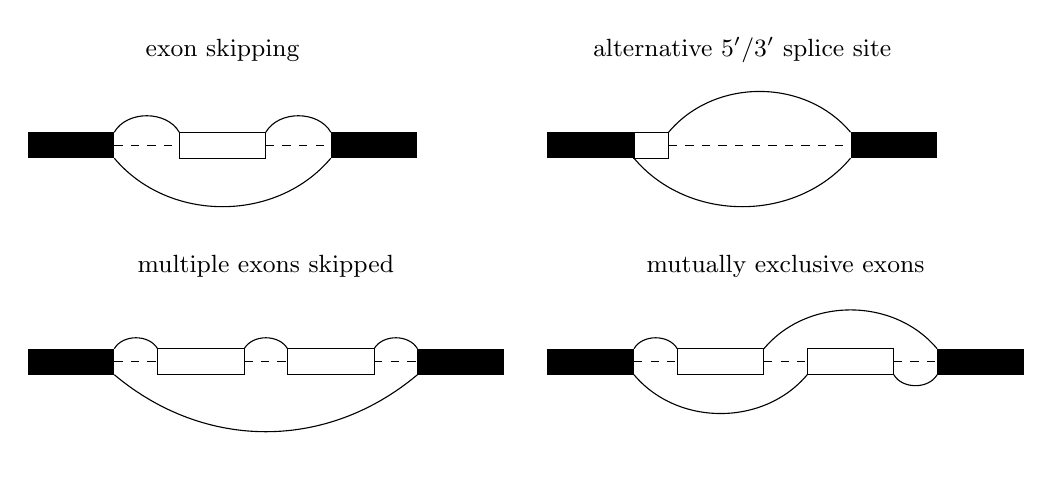
\begin{tikzpicture}[every node/.style={font=\small}, x=0.55cm, y=0.55cm]
    \tikzset{con/.style={fill=black}, alt/.style={fill=white, draw=black}}
    % exon skipping
    \begin{scope}[shift={(0,0)}]
      \node at (4.5,2.2) {exon skipping};
      \fill[con] (0,-0.3) rectangle (2,0.3); \draw[alt] (3.5,-0.3) rectangle (5.5,0.3); \fill[con] (7,-0.3) rectangle (9,0.3);
      \draw[dashed] (2,0) -- (3.5,0); \draw[dashed] (5.5,0) -- (7,0);
      \draw (2,0.3) to[out=60, in=120] (3.5,0.3); \draw (5.5,0.3) to[out=60, in=120] (7,0.3);
      \draw (2,-0.3) to[out=-50, in=-130] (7,-0.3);
    \end{scope}
    % alternative splice site
    \begin{scope}[shift={(12,0)}]
      \node at (4.5,2.2) {alternative $5'$/$3'$ splice site};
      \fill[con] (0,-0.3) rectangle (2,0.3); \draw[alt] (2,-0.3) rectangle (2.8,0.3); \fill[con] (7,-0.3) rectangle (9,0.3);
      \draw[dashed] (2.8,0) -- (7,0);
      \draw (2.8,0.3) to[out=50, in=130] (7,0.3);
      \draw (2,-0.3) to[out=-50, in=-130] (7,-0.3);
    \end{scope}
    % multiple exons skipped
    \begin{scope}[shift={(0,-5)}]
      \node at (5.5,2.2) {multiple exons skipped};
      \fill[con] (0,-0.3) rectangle (2,0.3); \draw[alt] (3,-0.3) rectangle (5,0.3); \draw[alt] (6,-0.3) rectangle (8,0.3); \fill[con] (9,-0.3) rectangle (11,0.3);
      \draw[dashed] (2,0) -- (3,0); \draw[dashed] (5,0) -- (6,0); \draw[dashed] (8,0) -- (9,0);
      \draw (2,0.3) to[out=60, in=120] (3,0.3); \draw (5,0.3) to[out=60, in=120] (6,0.3); \draw (8,0.3) to[out=60, in=120] (9,0.3);
      \draw (2,-0.3) to[out=-40, in=-140] (9,-0.3);
    \end{scope}
    % mutually exclusive
    \begin{scope}[shift={(12,-5)}]
      \node at (5.5,2.2) {mutually exclusive exons};
      \fill[con] (0,-0.3) rectangle (2,0.3); \draw[alt] (3,-0.3) rectangle (5,0.3); \draw[alt] (6,-0.3) rectangle (8,0.3); \fill[con] (9,-0.3) rectangle (11,0.3);
      \draw[dashed] (2,0) -- (3,0); \draw[dashed] (5,0) -- (6,0); \draw[dashed] (8,0) -- (9,0);
      \draw (2,0.3) to[out=60, in=120] (3,0.3); \draw (5,0.3) to[out=50, in=130] (9,0.3);
      \draw (2,-0.3) to[out=-50, in=-130] (6,-0.3); \draw (8,-0.3) to[out=-60, in=-120] (9,-0.3);
    \end{scope}
  \end{tikzpicture}
  \caption{Common types of alternative splicing. Black boxes are constitutive exons, white boxes alternative exonic sequence, dashed lines introns, and arcs the splice junctions joining exons in different isoforms. Junctions above and below each gene belong to different isoforms.}
  \label{fig:as_types}
\end{figure}

\paragraph{Splicing and disease.} Splicing is disrupted in many diseases. Some mutations destroy or create splice sites in a single gene, as in FTDP-17. Others hit the splicing machinery itself: recurrent mutations in splicing factors such as SF3B1, SRSF2 and U2AF1 drive myelodysplastic syndromes and some leukaemias~\citep{desterro2020}. In amyotrophic lateral sclerosis (ALS) and related neurodegenerative diseases, loss of the RNA-binding protein TDP-43 from the nucleus leads to widespread splicing errors, including the inclusion of \emph{cryptic exons}, intronic sequences that are normally never included. This makes splicing both a target for diagnosis and, increasingly, for therapy.

%======================================================================
\section{Measuring isoforms with RNA-seq}
\label{sec:rnaseq_isoforms}
%======================================================================

\subsection{Split reads}

Recall the RNA-seq protocol of Chapter 1. RNA is extracted from a sample, fragmented and reverse transcribed into complementary DNA (cDNA), and the cDNA fragments are sequenced to give reads of typically 100--150\,nt, which are aligned to the genome. Most of the RNA in a typical library is mature mRNA, from which the introns have already been removed. A read from a mature mRNA can therefore cross an exon-exon junction: it is contiguous in the transcript but not in the genome, and its alignment is split across two exons (Figure~\ref{fig:split_reads}). These \emph{split} or \emph{junction} reads are direct evidence that a particular pair of splice sites was joined, and they are the main source of information about splicing in short-read data. Aligners designed for RNA-seq, such as STAR~\citep{dobin2013}, search for such split alignments.

\begin{figure}[!htbp]
  \centering
  \begin{tikzpicture}[>=Stealth, every node/.style={font=\small}]
    \node[left] at (0,2.0) {mature mRNA};
    \draw[fill=blue!40] (0,1.85) rectangle (2.0,2.15);
    \draw[fill=green!40] (2.0,1.85) rectangle (3.2,2.15);
    \draw[fill=red!35] (3.2,1.85) rectangle (5.2,2.15);
    \foreach \x/\y in {0.3/2.35, 1.6/2.35, 2.9/2.6, 4.2/2.35} \draw[very thick] (\x,\y) -- (\x+0.8,\y);
    \node[right] at (5.4,2.45) {reads};
    \draw[->, thick] (2.6,1.7) -- (2.6,1.05) node[midway, right] {align to genome};
    \node[left] at (0,0) {genome};
    \draw (0,0) -- (11.4,0);
    \draw[fill=blue!40] (0,-0.15) rectangle (2.0,0.15);
    \draw[fill=green!40] (4.6,-0.15) rectangle (5.8,0.15);
    \draw[fill=red!35] (9.4,-0.15) rectangle (11.4,0.15);
    % unspliced reads
    \draw[very thick] (0.3,0.35) -- (1.1,0.35);
    \draw[very thick] (10.0,0.35) -- (10.8,0.35);
    % split reads
    \draw[very thick] (1.6,0.35) -- (2.0,0.35); \draw[densely dotted] (2.0,0.35) -- (4.6,0.35); \draw[very thick] (4.6,0.35) -- (5.0,0.35);
    \draw[very thick] (5.5,0.6) -- (5.8,0.6); \draw[densely dotted] (5.8,0.6) -- (9.4,0.6); \draw[very thick] (9.4,0.6) -- (9.9,0.6);
    \node[above, font=\footnotesize] at (3.3,0.35) {split read};
    \node[above, font=\footnotesize] at (7.6,0.6) {split read};
  \end{tikzpicture}
  \caption{Reads from a mature mRNA that cross an exon-exon junction align to the genome in two pieces, separated by the intron (dotted). These split reads show which splice sites were joined.}
  \label{fig:split_reads}
\end{figure}

\subsection{The isoform quantification problem}

Reads are much shorter than isoforms, which are typically thousands of nucleotides long, and different isoforms of a gene share most of their sequence. A read therefore usually cannot be assigned to a single isoform. Figure~\ref{fig:read_ambiguity} shows a gene with three isoforms and five reads. Read a lies in a region shared by all three isoforms; read b is compatible with the blue and green isoforms; read c with blue and red; read e with green and red. Only read d, a split read joining two exons that are adjacent only in the red isoform, identifies its isoform uniquely.

\begin{figure}[!htbp]
  \centering
  \begin{tikzpicture}[every node/.style={font=\small}]
    \tikzset{iso/.style={line width=3pt}}
    % isoforms: E1 [0,3), E1s [0,1.5), E2 [5,7), E3 [10,13) scaled by 0.6
    \begin{scope}[x=0.6cm]
      \draw[iso, blue!80!black] (0,0) -- (3,0); \draw[dotted, thick] (3,0) -- (5,0); \draw[iso, blue!80!black] (5,0) -- (7,0);
      \node[left] at (-0.2,0) {blue};
      \draw[iso, green!60!black] (0,-0.6) -- (3,-0.6); \draw[dotted, thick] (3,-0.6) -- (10,-0.6); \draw[iso, green!60!black] (10,-0.6) -- (13,-0.6);
      \node[left] at (-0.2,-0.6) {green};
      \draw[iso, red!80!black] (0,-1.2) -- (1.5,-1.2); \draw[dotted, thick] (1.5,-1.2) -- (5,-1.2); \draw[iso, red!80!black] (5,-1.2) -- (7,-1.2); \draw[dotted, thick] (7,-1.2) -- (10,-1.2); \draw[iso, red!80!black] (10,-1.2) -- (13,-1.2);
      \node[left] at (-0.2,-1.2) {red};
      \draw (0,-1.8) -- (13,-1.8); \node[right] at (13.1,-1.8) {genome};
      % reads
      \draw[very thick] (0.3,0.7) -- (1.3,0.7) node[midway, below=1pt] {a};
      \draw[very thick] (1.8,0.7) -- (2.8,0.7) node[midway, below=1pt] {b};
      \draw[very thick] (5.5,0.7) -- (6.5,0.7) node[midway, below=1pt] {c};
      \draw[very thick] (6.5,1.5) -- (7,1.5); \draw (7,1.5) -- (10,1.5); \draw[very thick] (10,1.5) -- (10.5,1.5);
      \node[below=1pt] at (8.5,1.5) {d};
      \draw[very thick] (11.3,0.7) -- (12.3,0.7) node[midway, below=1pt] {e};
      % pies
      \newcommand{\readpie}[4]{%
        \begin{scope}[shift={(#1,#2)}]
          \foreach \c/\s/\e in {#3} \fill[\c] (0,0) -- (\s:0.25) arc[start angle=\s, end angle=\e, radius=0.25] -- cycle;
          \draw (0,0) circle (0.25);
        \end{scope}}
      \readpie{0.8}{1.3}{blue!80!black/90/210, green!60!black/210/330, red!80!black/330/450}{}
      \readpie{2.3}{1.3}{blue!80!black/90/270, green!60!black/270/450}{}
      \readpie{6.0}{1.3}{blue!80!black/90/270, red!80!black/270/450}{}
      \readpie{8.5}{2.2}{red!80!black/0/360}{}
      \readpie{11.8}{1.3}{green!60!black/90/270, red!80!black/270/450}{}
    \end{scope}
  \end{tikzpicture}
  \caption{Ambiguity in assigning short reads to isoforms, after \citet{pachter2011}. Three isoforms of a gene (coloured lines; dotted segments are introns) and five aligned reads. The pie above each read shows the isoforms it is compatible with. Only the split read d is unique to one isoform.}
  \label{fig:read_ambiguity}
\end{figure}

We want to know two things: how abundant each isoform is, and which isoform each read came from. The two problems are coupled. If we knew which isoform each read came from, we could estimate abundances by counting. Conversely, if we knew the abundances, we could assign each read probabilistically: if the green and red isoforms were barely expressed, read a would most likely come from the blue isoform. This is the structure of a latent variable problem, the assignments being latent, and like the clustering problems of Chapter 5 it is solved by EM~\citep{trapnell2010,li2011rsem,pachter2011,bray2016}.

Real genes can be much more complicated than this cartoon. Figure~\ref{fig:neurexin} shows the isoforms of neurexin 1$\alpha$, a synaptic protein implicated in neurodevelopmental and psychiatric disorders, sequenced as full-length molecules with long reads: 247 distinct isoforms were found among 2,574 sequenced transcripts, produced by combinations of alternative exons that encode parts of different protein domains~\citep{treutlein2014}. Inferring such a repertoire from short reads is very poorly determined.

\begin{figure}[!htbp]
  \centering
  \includegraphics[width=0.6\linewidth]{slides/neurexin_isoforms.jpg}
  \caption{Splice isoforms of mouse neurexin 1$\alpha$ (\textit{Nrxn1}$\alpha$) observed by single-molecule long-read sequencing of full-length mRNAs. Rows are the 247 distinct isoforms and columns are exons, coloured green if included; the bar graph on the right gives the number of transcripts observed for each isoform, and the protein domains encoded by the exons are shown at the top. Reproduced from \citet{treutlein2014}.}
  \label{fig:neurexin}
\end{figure}

%======================================================================
\section{A generative model for RNA-seq reads}
\label{sec:generative}
%======================================================================

\subsection{The model}

Most isoform quantification methods use a variant of the following generative model~\citep{glaus2012,nariai2013,hensman2015}. Let $N$ be the number of reads and $M$ the number of isoforms, indexed by $n\in\{1,\dots,N\}$ and $m\in\{1,\dots,M\}$. In a whole transcriptome $M$ is of the order of $10^5$, since the roughly 20,000 human protein-coding genes have several annotated isoforms each, and $N$ is tens of millions. Let $\vtheta=(\theta_1,\dots,\theta_M)$ be a probability vector, $\theta_m\geq 0$ and $\sum_m\theta_m=1$, where $\theta_m$ is the probability that a randomly chosen read comes from isoform $m$. Let $t_n\in\{1,\dots,M\}$ be the isoform that read $n$ came from, and $r_n$ the observed read (its sequence and alignment). The model is
\begin{align}
  \vtheta &\sim \Dir(\valpha), \nonumber\\
  t_n\mid\vtheta &\sim \Disc(\vtheta), \qquad n=1,\dots,N, \label{eq:genmodel}\\
  r_n\mid t_n &\sim p(r_n\mid t_n), \nonumber
\end{align}
where $\valpha\in\R_{>0}^M$ is the parameter of a Dirichlet prior (Section~\ref{sec:dirichlet}) and $\Disc(\vtheta)$ is the discrete (categorical) distribution with $p(t_n=m\mid\vtheta)=\theta_m$. The prior encodes the intuition that an isoform that makes up more of the RNA is, a priori, more likely to be the source of any given read.

The last line is the \emph{read likelihood}. We do not model the read sequence in detail. Instead, we write $p_{nm}=p(r_n\mid t_n=m)$ for the probability of observing exactly read $n$ given that it came from isoform $m$. In the simplest version, a read of length $l$ is equally likely to start at any position of the isoform, and isoform $m$, of length $L_m$, has
\begin{equation}
  \tilde L_m = L_m - l + 1
\end{equation}
possible start positions: place the read at the start of the isoform and slide it one position at a time until it reaches the end. $\tilde L_m$ is called the \emph{effective length}. If read $n$ aligns to isoform $m$ at one of these positions, it is one of $\tilde L_m$ equally likely reads, so
\begin{equation}
  p_{nm} = \frac{y_{nm}}{\tilde L_m}, \qquad
  y_{nm} = \begin{cases} 1 & \text{if read $n$ is compatible with isoform $m$},\\ 0 & \text{otherwise}. \end{cases}
  \label{eq:readlik}
\end{equation}
The values $p_{nm}$ are computed once from the alignments and stay fixed; only $\vtheta$ and the $t_n$ are unknown. Practical methods refine~\eqref{eq:readlik} with the distribution of fragment lengths for paired-end reads, sequencing error probabilities, and biases in where fragments start along the transcript~\citep{li2011rsem,glaus2012,patro2017}, but these only change the values of $p_{nm}$.

Because a long isoform yields more reads than a short one present in the same number of copies, $\theta_m$ is the share of \emph{reads}, not of molecules. If $\tau_m$ is the fraction of RNA molecules that are isoform $m$, then $\theta_m\propto\tau_m\tilde L_m$, and conversely
\begin{equation}
  \tau_m = \frac{\theta_m/\tilde L_m}{\sum_{m'}\theta_{m'}/\tilde L_{m'}} .
\end{equation}
Multiplying $\tau_m$ by $10^6$ gives the familiar unit of transcripts per million (TPM).

\paragraph{Indicator notation.} It helps to encode $t_n$ as a one-hot vector $\vz_n\in\{0,1\}^M$ with $z_{nm}=\ind[t_n=m]$, where $\ind[\cdot]$ is the indicator function, so that $\sum_m z_{nm}=1$. Then $p(t_n\mid\vtheta)=\theta_{t_n}=\prod_m\theta_m^{z_{nm}}$. The product picks out the right element because $\theta^0=1$ and $\theta^1=\theta$: every factor except the one for $m=t_n$ equals one. Similarly $p(r_n\mid t_n)=p_{nt_n}=\prod_m p_{nm}^{z_{nm}}$. Writing $\mZ\in\{0,1\}^{N\times M}$ for the matrix with rows $\vz_n^\top$ and $R=\{r_1,\dots,r_N\}$ for the reads, the joint distribution of all variables is the product of the three terms of~\eqref{eq:genmodel},
\begin{equation}
  p(\vtheta,\mZ,R) = \underbrace{\frac{\Gamma(\alpha_\cdot)}{\prod_m\Gamma(\alpha_m)}\prod_{m=1}^M\theta_m^{\alpha_m-1}}_{\text{Dirichlet prior}}\;
  \underbrace{\prod_{n=1}^N\prod_{m=1}^M\theta_m^{z_{nm}}}_{\text{read origins}}\;
  \underbrace{\prod_{n=1}^N\prod_{m=1}^M p_{nm}^{z_{nm}}}_{\text{read likelihood}},
  \label{eq:joint}
\end{equation}
where $\Gamma$ is the gamma function and $\alpha_\cdot=\sum_m\alpha_m$.

\subsection{The Dirichlet distribution}
\label{sec:dirichlet}

The Dirichlet distribution is the standard distribution over probability vectors, in the way the Gaussian is the standard distribution over real vectors. For $K$ categories, its random variable is a vector $\vpi\in\R^K$ in the \emph{probability simplex}
\begin{equation}
  \simplex^{K-1} = \Big\{\vpi\in\R^K : \pi_k\geq 0,\ \textstyle\sum_{k=1}^K\pi_k=1\Big\},
\end{equation}
which has dimension $K-1$ because of the sum constraint. Its parameter is a vector $\va\in\R_{>0}^K$, and its density is
\begin{equation}
  \Dir(\vpi;\va) = \frac{\Gamma(a_\cdot)}{\prod_{k=1}^K\Gamma(a_k)}\prod_{k=1}^K\pi_k^{a_k-1}, \qquad a_\cdot=\sum_{k=1}^K a_k ,
  \label{eq:dirichlet}
\end{equation}
where the dot subscript denotes a sum over the index. The ratio of gamma functions is the normalizing constant; the dependence on $\vpi$ is the simple product $\prod_k\pi_k^{a_k-1}$. For $K=2$ the Dirichlet is the beta distribution. Its main properties are:
\begin{itemize}
  \item mean $\E[\pi_k]=a_k/a_\cdot$, the normalized parameter vector;
  \item mode $(a_k-1)/(a_\cdot-K)$, the normalized vector $\va-\mathbf{1}$, provided all $a_k>1$;
  \item variance $\operatorname{Var}[\pi_k]=\dfrac{a_k(a_\cdot-a_k)}{a_\cdot^2(a_\cdot+1)}$;
  \item $\E[\log\pi_k]=\psi(a_k)-\psi(a_\cdot)$, where $\psi(x)=\frac{d}{dx}\log\Gamma(x)$ is the digamma function.
\end{itemize}
The mean suggests a second parameterization, $\va=c\vp$, where $\vp\in\simplex^{K-1}$ is the mean and the scalar $c=a_\cdot>0$ is the \emph{concentration}. The variance becomes $p_k(1-p_k)/(c+1)$, so larger $c$ concentrates the distribution around its mean.

Figure~\ref{fig:dirichlet_simplex} shows Dirichlet densities for $K=3$. The simplex $\simplex^2$ is a triangle in $\R^3$ with corners at $(1,0,0)$, $(0,1,0)$ and $(0,0,1)$; we view it face on, and the distance from a point to each edge is the corresponding component. With $\va=(1,1,1)$, that is $c=3$ and $\vp=(\frac13,\frac13,\frac13)$, the density is uniform. Increasing $c$ concentrates the mass around the centre, and changing $\vp$ moves it. Figure~\ref{fig:dirichlet_draws} shows draws for $K=10$. With $c=100$ a draw is close to its mean; with $c=3$ it is far from it, and many components are close to zero. When some $a_k<1$ (for a uniform mean, when $c<K$), the density becomes infinite at the edges of the simplex and draws are sparse, with most of their mass on a few components.

\begin{figure}[!htbp]
  \centering
  \includegraphics[width=0.95\linewidth]{dirichlet_simplex.pdf}
  \caption{Dirichlet densities on the simplex $\simplex^2$, viewed face on, for parameter $\va=c\vp$. The first three panels have mean $\vp=(\frac13,\frac13,\frac13)$ (cross) and increasing concentration $c$; $c=3$ gives the uniform distribution. The last has mean $(0.6,0.2,0.2)$, nearest the corner where $\pi_1=1$. Lighter colours indicate higher density.}
  \label{fig:dirichlet_simplex}
\end{figure}

\begin{figure}[!htbp]
  \centering
  \includegraphics[width=0.95\linewidth]{dirichlet_draws.pdf}
  \caption{Single draws from $\Dir(c\vp)$ with $K=10$, for a uniform mean (left) and a non-uniform mean (right, top row), at concentrations $c=100$, 30 and 3. As $c$ decreases, draws move further from the mean and become sparse.}
  \label{fig:dirichlet_draws}
\end{figure}

The Dirichlet is the \emph{conjugate prior} of the discrete distribution: if $\vpi\sim\Dir(\va)$ and we observe $n_k$ draws of category $k$ from $\Disc(\vpi)$, the posterior is $\Dir(\va+\mathbf{n})$, where $\mathbf{n}=(n_1,\dots,n_K)$. This follows from multiplying~\eqref{eq:dirichlet} by the likelihood $\prod_k\pi_k^{n_k}$, which gives $\prod_k\pi_k^{a_k+n_k-1}$. The parameter $a_k$ therefore acts as a pseudo-count, and $\va=\mathbf{1}$ adds no pseudo-counts at all. In the isoform model, if we knew the read origins $\mZ$, the posterior of $\vtheta$ would be $\Dir(\valpha+\sum_n\vz_n)$. Conjugacy will make every update in the next two sections available in closed form.

\subsection{Graphical model}

Figure~\ref{fig:graphical_model-10} shows the model as a directed graphical model, a notation we used for hidden Markov models in Chapter 6. Each node is a random variable, an edge means that the distribution of the child depends on the parent, and shaded nodes are observed. The rectangles are \emph{plates}: the variables inside a plate are repeated the number of times shown in its corner, like the body of a for loop, and plates can be nested like nested loops. There is one $z_{nm}$ for every read and every isoform, $N\times M$ in total, and one observed read $r_n$ per read. Each $z_{nm}$ depends on $\vtheta$, and each $r_n$ depends on $\vz_n$.

\begin{figure}[!htbp]
  \centering
  \begin{tikzpicture}[>=Stealth, every node/.style={font=\small},
      var/.style={circle, draw, minimum size=0.9cm}, obs/.style={var, fill=gray!25}]
    \node[var] (alpha) at (-2.0,0) {$\valpha$};
    \node[var] (theta) at (0,0) {$\vtheta$};
    \node[var] (z) at (2.8,0) {$z_{nm}$};
    \node[obs] (r) at (2.8,-2.0) {$r_n$};
    \draw[->] (alpha) -- (theta);
    \draw[->] (theta) -- (z);
    \draw[->] (z) -- (r);
    \node[draw, rounded corners, fit=(z), inner sep=0.35cm, label={[anchor=south east]south east:$M$}] (pm) {};
    \node[draw, rounded corners, fit=(pm)(r), inner sep=0.3cm, label={[anchor=south east]south east:$N$}] {};
  \end{tikzpicture}
  \caption{Graphical model for isoform quantification, adapted from \citet{hensman2015}. Plates denote repetition over isoforms $m$ and reads $n$; the shaded node is observed. The quantity of interest is the posterior $p(\vtheta\mid R)$.}
  \label{fig:graphical_model-10}
\end{figure}

What we would like is the posterior $p(\vtheta\mid R)$. Obtaining it requires summing the joint~\eqref{eq:joint} over the latent assignments $\mZ$. The sum over the assignment of each read is easy, but the posterior over $\vtheta$ that results, $p(\vtheta\mid R)\propto\Dir(\vtheta;\valpha)\prod_n\sum_m\theta_m p_{nm}$, is a product of $N$ sums. Expanding it gives a mixture of up to $M^N$ Dirichlet distributions, one per joint assignment of reads to isoforms, which cannot be computed. We consider two ways around this: point estimation of $\vtheta$ by EM, and approximation of the full posterior by variational inference.

%======================================================================
\section{EM for isoform abundance}
\label{sec:em-10}
%======================================================================

EM was derived in Chapter 5 for mixture models and used in Chapter 6 for hidden Markov models. It maximizes a lower bound on the log marginal probability of the data by alternating two steps: the E step sets a distribution $q(\mZ)$ over the latent variables to their posterior given the current parameters, and the M step maximizes the expected log joint probability under $q$ over the parameters. Here the latent variables are the read assignments $\mZ$ and the parameter is $\vtheta$. Because we keep the Dirichlet prior, the M step maximizes the expected log \emph{posterior} and EM finds a maximum a posteriori (MAP) estimate of $\vtheta$; with $\valpha=\mathbf{1}$ the prior is flat and the estimate is the maximum likelihood estimate.

\subsection{E step}

The E step computes the posterior over the assignments given the current $\vtheta$. Only the second and third factors of~\eqref{eq:joint} involve $\mZ$, and they factorize over reads, so the assignments of different reads are independent given $\vtheta$ and
\begin{equation}
  q(\vz_n) = p(\vz_n\mid r_n,\vtheta) \propto \prod_{m=1}^M\theta_m^{z_{nm}}p_{nm}^{z_{nm}} = \prod_{m=1}^M\left(\theta_m p_{nm}\right)^{z_{nm}} .
\end{equation}
This is the probability mass function of a discrete distribution over which entry of $\vz_n$ equals one, with unnormalized probabilities $\phi^*_{nm}=\theta_m p_{nm}$. Normalizing,
\begin{equation}
  q(\vz_n) = \prod_{m=1}^M\phi_{nm}^{z_{nm}}, \qquad
  \phi_{nm} = \frac{\theta_m p_{nm}}{\sum_{m'=1}^M\theta_{m'}p_{nm'}} ,
  \label{eq:estep}
\end{equation}
where $\phi_{nm}\in[0,1]$, with $\sum_m\phi_{nm}=1$, is the posterior probability that read $n$ came from isoform $m$, also called its \emph{responsibility}. The general pattern is worth noting. Collect the terms of the joint that involve the variable of interest, recognize the result as the unnormalized form of a standard distribution, and read off its parameters. The same pattern recurs in the M step and in variational inference.

\subsection{M step}

The M step maximizes the expected log joint under $q(\mZ)=\prod_n q(\vz_n)$. Taking the log of~\eqref{eq:joint},
\begin{equation}
  \log p(\vtheta,\mZ,R) = \sum_{m=1}^M(\alpha_m-1)\log\theta_m + \sum_{n=1}^N\sum_{m=1}^M z_{nm}\log\theta_m + \sum_{n=1}^N\sum_{m=1}^M z_{nm}\log p_{nm} + \text{const},
\end{equation}
where the constant is the log normalizer of the Dirichlet, which does not involve $\vtheta$. Expectation is linear, so it moves inside the sums, and $\E_q[z_{nm}]=\phi_{nm}$ because $z_{nm}$ is one with probability $\phi_{nm}$ and zero otherwise. Dropping terms that do not involve $\vtheta$ and exchanging the order of the sums over $n$ and $m$,
\begin{equation}
  \E_q\left[\log p(\vtheta,\mZ,R)\right] = \sum_{m=1}^M\Big(\alpha_m-1+\sum_{n=1}^N\phi_{nm}\Big)\log\theta_m + \text{const}
  = \sum_{m=1}^M(\alpha'_m-1)\log\theta_m + \text{const},
\end{equation}
with
\begin{equation}
  \alpha'_m = \alpha_m + \sum_{n=1}^N\phi_{nm} .
  \label{eq:alphaprime}
\end{equation}
Up to a constant this is the log density of $\Dir(\vtheta;\valpha')$, so the M step returns its mode. To derive the mode, maximize $\sum_m(\alpha'_m-1)\log\theta_m$ subject to $\sum_m\theta_m=1$ with a Lagrange multiplier $\lambda$. Setting the derivative of $\sum_m(\alpha'_m-1)\log\theta_m-\lambda(\sum_m\theta_m-1)$ with respect to $\theta_m$ to zero gives $(\alpha'_m-1)/\theta_m=\lambda$, so $\theta_m=(\alpha'_m-1)/\lambda$, and the constraint gives $\lambda=\sum_m(\alpha'_m-1)=\alpha_\cdot-M+N$, using $\sum_n\sum_m\phi_{nm}=N$. The M step is therefore
\begin{equation}
  \theta_m^{\text{new}} = \frac{\alpha'_m-1}{\alpha'_\cdot-M} = \frac{\alpha_m-1+\sum_n\phi_{nm}}{N+\alpha_\cdot-M},
  \label{eq:mstep-10}
\end{equation}
which requires $\alpha'_m\geq 1$; for $\alpha_m<1$ the maximum can lie on the boundary $\theta_m=0$. With a flat prior, $\valpha=\mathbf{1}$, the update is $\theta_m^{\text{new}}=\frac{1}{N}\sum_n\phi_{nm}$.

The quantity $\sum_n\phi_{nm}$ is the \emph{expected count} of reads from isoform $m$, the analogue of the expected number of points in a cluster in EM for a Gaussian mixture. The algorithm alternates between dividing each read among the isoforms it is compatible with, in proportion to their current abundances weighted by $1/\tilde L_m$, and re-estimating the abundances from the resulting fractional counts (Algorithm~\ref{alg:em}).

\begin{algorithm}[!htbp]
  \caption{EM for isoform abundance}
  \label{alg:em}
  \begin{algorithmic}[1]
    \State Compute $p_{nm}=y_{nm}/\tilde L_m$ from the read alignments
    \State Initialize $\theta_m\gets 1/M$ for all $m$
    \Repeat
      \State E step: $\phi_{nm}\gets\theta_m p_{nm}/\sum_{m'}\theta_{m'}p_{nm'}$ for all $n,m$
      \State M step: $\theta_m\gets(\alpha_m-1+\sum_n\phi_{nm})/(N+\alpha_\cdot-M)$ for all $m$
    \Until{the log posterior $\log\Dir(\vtheta;\valpha)+\sum_n\log\sum_m\theta_m p_{nm}$ stops increasing}
    \State Return $\vtheta$, and $\tau_m\propto\theta_m/\tilde L_m$
  \end{algorithmic}
\end{algorithm}

\subsection{Properties}

As shown in Chapter 5, each EM iteration cannot decrease the objective, here the log posterior
\begin{equation}
  \log p(\vtheta\mid R) = \sum_{m=1}^M(\alpha_m-1)\log\theta_m + \sum_{n=1}^N\log\sum_{m=1}^M\theta_m p_{nm} + \text{const}.
\end{equation}
Unlike the Gaussian mixture, this objective is concave in $\vtheta$ when $\valpha\geq\mathbf{1}$: each $\sum_m\theta_m p_{nm}$ is linear in $\vtheta$, the logarithm of a linear function is concave, sums of concave functions are concave, and the simplex is convex. EM therefore converges to a global maximum, although it can be slow when isoforms are hard to distinguish, and the maximum need not be unique. If two isoforms are compatible with exactly the same reads, for example, only their combined abundance is determined by the data.

The E step depends on a read only through its vector $(p_{n1},\dots,p_{nM})$, which by~\eqref{eq:readlik} is determined by the set of isoforms the read is compatible with. Reads with the same compatibility set, an \emph{equivalence class}, have identical responsibilities, so the E step can be computed once per class and weighted by the number of reads in it. Fast methods such as kallisto~\citep{bray2016} and salmon~\citep{patro2017} exploit this, together with fast approximate alignment (pseudoalignment), to quantify tens of millions of reads in minutes.

Figure~\ref{fig:em_toy} runs EM on a simulated gene with the three-isoform structure of Figure~\ref{fig:read_ambiguity}. Starting from uniform abundances, the estimates converge within a few tens of iterations to the maximum likelihood estimate, which is close to the values used to simulate the data, and the log likelihood increases at every iteration.

\begin{figure}[!htbp]
  \centering
  \includegraphics[width=0.9\linewidth]{em_toy.pdf}
  \caption{EM for a simulated three-isoform gene with the structure of Figure~\ref{fig:read_ambiguity} ($N=1000$ reads of length $l=50$, flat prior). Left: estimated read proportions $\theta_m$ by iteration, with the values used to simulate the data dashed. Right: the log likelihood $\sum_n\log\sum_m\theta_m p_{nm}$ never decreases.}
  \label{fig:em_toy}
\end{figure}

%======================================================================
\section{Variational Bayesian inference}
\label{sec:vi}
%======================================================================

EM keeps a distribution over the read assignments $\mZ$, so it represents our uncertainty about which isoform each read came from, but it returns a single value of $\vtheta$. That can be misleading. An isoform supported by only a handful of reads, or one that can be distinguished from another only through a few junction reads, has an abundance we know poorly, and a point estimate does not say so. The Bayesian answer is the posterior $p(\vtheta\mid R)$, which we saw is intractable. \emph{Variational inference} approximates it: we choose a family of tractable distributions $q$ and find the member closest to the posterior. It replaces a hard integration problem with an optimization problem, which is usually easier in high dimensions.

\subsection{The evidence lower bound}

Consider a general model with latent variables $\vz$ (which may include parameters) and data $\vx$. By Bayes' rule the posterior is
\begin{equation}
  p(\vz\mid\vx) = \frac{p(\vx\mid\vz)\,p(\vz)}{p(\vx)} = \frac{f(\vz)}{C},
\end{equation}
where $f(\vz)=p(\vx,\vz)$ is the joint probability, which we can evaluate, and $C=p(\vx)=\int f(\vz)\,d\vz$ is the evidence or marginal likelihood, which we cannot. For any distribution $q(\vz)$, multiplying and dividing by $q$ inside the integral and applying Jensen's inequality to the concave logarithm, as in Chapter 5,
\begin{equation}
  \log C = \log\int q(\vz)\frac{f(\vz)}{q(\vz)}\,d\vz \geq \int q(\vz)\log\frac{f(\vz)}{q(\vz)}\,d\vz \equiv \mathcal{F}[q] .
\end{equation}
$\mathcal{F}[q]$ is the evidence lower bound (ELBO), or variational free energy. The gap is
\begin{equation}
  \log C - \mathcal{F}[q] = \int q(\vz)\left[\log C + \log\frac{q(\vz)}{f(\vz)}\right]d\vz = \int q(\vz)\log\frac{q(\vz)}{p(\vz\mid\vx)}\,d\vz = \KL\big(q\,\|\,p(\cdot\mid\vx)\big),
  \label{eq:vi_gap}
\end{equation}
using $\int q=1$ and $f/C=p(\vz\mid\vx)$. The Kullback-Leibler (KL) divergence $\KL(q\|p)=\int q\log(q/p)$ is non-negative and zero only when $q=p$. Since $\log C$ does not depend on $q$, maximizing $\mathcal{F}[q]$ over $q$ is the same as minimizing the KL divergence from $q$ to the posterior, and it requires only the joint $f$, not the evidence. EM is the special case in which $q$ is unrestricted over the latent variables and a point mass over the parameters.

\subsection{Which divergence?}

The KL divergence is not symmetric, and the direction matters. $\KL(q\|p)$ averages $\log(q/p)$ under $q$. Where $p$ is close to zero and $q$ is not, $\log(q/p)$ is very large, so the optimal $q$ avoids putting mass where the posterior has none. This is called \emph{zero forcing}. As a result, $q$ tends to fit one mode of a multimodal $p$ and ignore the others, which is called \emph{mode seeking}, and it tends to underestimate the spread of $p$. The reverse divergence $\KL(p\|q)$ penalizes $q$ for missing mass that $p$ has, so it spreads $q$ to cover all of $p$; for a Gaussian $q$ it matches the mean and variance of $p$. \citet{minka2005} placed both in the family of $\alpha$-divergences,
\begin{equation}
  D_\alpha(p\,\|\,q) = \frac{1}{\alpha(1-\alpha)}\int\left[\alpha p(\vz)+(1-\alpha)q(\vz)-p(\vz)^\alpha q(\vz)^{1-\alpha}\right]d\vz,
\end{equation}
which tends to $\KL(q\|p)$ as $\alpha\to 0$ and to $\KL(p\|q)$ as $\alpha\to 1$, with intermediate values interpolating between zero forcing and mass covering (Figure~\ref{fig:kl_directions}). Standard variational inference uses $\KL(q\|p)$, the one direction in which the expectation is under the tractable $q$; expectation propagation uses the other.

\begin{figure}[!htbp]
  \centering
  \includegraphics[width=0.95\linewidth]{kl_directions.pdf}
  \caption{The Gaussian $q$ (red) that minimizes the $\alpha$-divergence $D_\alpha(p\|q)$ to a bimodal $p$ (blue), found numerically. $\alpha\to0$ gives $\KL(q\|p)$, used by variational inference, which locks onto one mode (zero forcing); $\alpha=1$ gives $\KL(p\|q)$, which matches the mean and variance of $p$ and covers both modes.}
  \label{fig:kl_directions}
\end{figure}

\subsection{Mean-field approximation and coordinate ascent}

The family of approximating distributions must be simple enough that $\mathcal{F}[q]$ can be computed. In \emph{mean-field} variational inference (the name comes from statistical physics) we assume $q$ factorizes over groups of variables,
\begin{equation}
  q(\vz) = \prod_{i=1}^I q_i(\vz_i),
\end{equation}
where $\vz_1,\dots,\vz_I$ partition $\vz$, and we make no other assumption about the form of the factors. The true posterior has dependencies between the groups; in the isoform model, for instance, the components of $\vtheta$ must sum to one, so if one is larger the others must be smaller. The factorized $q$ ignores such dependencies.

The factors can be optimized one at a time, holding the others fixed. Write $q_{-i}=\prod_{j\neq i}q_j$ and $\E_{-i}$ for expectation under $q_{-i}$. Separating the terms of $\mathcal{F}$ that involve $q_i$,
\begin{equation}
  \mathcal{F}[q] = \int q_i(\vz_i)\,\E_{-i}\left[\log f(\vz)\right]d\vz_i - \int q_i(\vz_i)\log q_i(\vz_i)\,d\vz_i + \text{const},
\end{equation}
where the constant collects the entropies of the other factors. Define the distribution
\begin{equation}
  \tilde p_i(\vz_i) = \frac{1}{Z_i}\exp\E_{-i}\left[\log f(\vz)\right],
\end{equation}
where $Z_i$ is its normalizing constant. Then the first two terms equal $-\KL(q_i\|\tilde p_i)+\log Z_i$, which is maximized by $q_i=\tilde p_i$. This gives the \emph{coordinate ascent variational inference} (CAVI) update~\citep{blei2017}, also known as variational Bayes EM,
\begin{equation}
  q_i^{\text{new}}(\vz_i) \propto \exp\left(\int\log f(\vz)\prod_{j\neq i}q_j(\vz_j)\,d\vz_{-i}\right) = \exp\,\E_{-i}\left[\log p(\vx,\vz)\right].
  \label{eq:cavi}
\end{equation}
Cycling through the factors increases $\mathcal{F}$ at every step, so CAVI converges to a local maximum of the ELBO.

\subsection{CAVI for isoform abundance}

For the isoform model we treat both $\vtheta$ and $\mZ$ as unknowns and assume
\begin{equation}
  q(\vtheta,\mZ) = q(\vtheta)\prod_{n=1}^N q(\vz_n),
\end{equation}
that is, abundances independent of assignments, and assignments of different reads independent of each other. Given $\vtheta$ the reads are independent anyway, so the only approximation is the independence of $\vtheta$ and $\mZ$.

\paragraph{Update for $q(\vz_n)$.} The terms of the log joint $\log p(\vtheta,\mZ,R)$ that involve $\vz_n$ are $\sum_m z_{nm}(\log\theta_m+\log p_{nm})$, so by~\eqref{eq:cavi}
\begin{equation}
  q^{\text{new}}(\vz_n) \propto \exp\,\E_{q(\vtheta)}\Big[\sum_{m=1}^M z_{nm}\log\theta_m + z_{nm}\log p_{nm}\Big] = \prod_{m=1}^M\left(p_{nm}e^{\E[\log\theta_m]}\right)^{z_{nm}},
\end{equation}
a discrete distribution, $q(\vz_n)=\prod_m\phi_{nm}^{z_{nm}}$, with
\begin{equation}
  \phi_{nm} = \frac{p_{nm}\exp(\E_{q(\vtheta)}[\log\theta_m])}{\sum_{m'}p_{nm'}\exp(\E_{q(\vtheta)}[\log\theta_{m'}])} .
  \label{eq:vb_phi}
\end{equation}
This is the E step~\eqref{eq:estep} with $\theta_m$ replaced by $\exp\E[\log\theta_m]$.

\paragraph{Update for $q(\vtheta)$.} The terms involving $\vtheta$ are the Dirichlet prior and the read origins. Taking the expectation under $q(\mZ)$, with $\E[z_{nm}]=\phi_{nm}$,
\begin{equation}
  q^{\text{new}}(\vtheta) \propto \exp\,\E_{q(\mZ)}\Big[\sum_m(\alpha_m-1)\log\theta_m + \sum_n\sum_m z_{nm}\log\theta_m\Big] = \prod_{m=1}^M\theta_m^{\alpha'_m-1},
\end{equation}
with $\alpha'_m=\alpha_m+\sum_n\phi_{nm}$ as in~\eqref{eq:alphaprime}. This is the kernel of a Dirichlet, so $q(\vtheta)=\Dir(\vtheta;\valpha')$. The computation is the same as in the M step; the only difference is that we exponentiate rather than maximize, and so keep the whole distribution rather than its mode. The expectation needed in~\eqref{eq:vb_phi} then has a closed form,
\begin{equation}
  \E_{q(\vtheta)}[\log\theta_m] = \psi(\alpha'_m) - \psi(\alpha'_\cdot).
\end{equation}

We assumed only the factorization. That $q(\vz_n)$ came out discrete and $q(\vtheta)$ came out Dirichlet was not assumed: it follows from~\eqref{eq:cavi} because the Dirichlet prior is conjugate to the discrete distribution of the read origins. The model is \emph{conditionally conjugate}: each variable's conditional distribution given the others is in the same family as its prior.

Algorithm~\ref{alg:cavi} collects the updates. Convergence can be monitored with the ELBO. Substituting the factors into $\mathcal{F}=\E_q[\log p(\vtheta,\mZ,R)]-\E_q[\log q(\vtheta)]-\sum_n\E_q[\log q(\vz_n)]$, the terms in $\E[\log\theta_m]$ cancel once $\valpha'=\valpha+\sum_n\vphi_n$, leaving
\begin{equation}
  \mathcal{F} = \log\frac{\Gamma(\alpha_\cdot)}{\Gamma(\alpha'_\cdot)} + \sum_{m=1}^M\log\frac{\Gamma(\alpha'_m)}{\Gamma(\alpha_m)} + \sum_{n=1}^N\sum_{m=1}^M\phi_{nm}\log\frac{p_{nm}}{\phi_{nm}} .
\end{equation}

\begin{algorithm}[!htbp]
  \caption{CAVI for isoform abundance}
  \label{alg:cavi}
  \begin{algorithmic}[1]
    \State Compute $p_{nm}$ from the alignments; initialize $\valpha'\gets\valpha+N/M$
    \Repeat
      \State $\phi_{nm}\gets p_{nm}\exp(\psi(\alpha'_m)-\psi(\alpha'_\cdot))$, then normalize over $m$, for all $n$
      \State $\alpha'_m\gets\alpha_m+\sum_n\phi_{nm}$ for all $m$
    \Until{the ELBO $\mathcal{F}$ stops increasing}
    \State Return $q(\vtheta)=\Dir(\valpha')$, with posterior mean $\alpha'_m/\alpha'_\cdot$
  \end{algorithmic}
\end{algorithm}

The update has a simple interpretation. For large $x$, $\exp(\psi(x))\approx x-\frac12$, so for well-supported isoforms $\exp\E[\log\theta_m]\approx(\alpha'_m-\frac12)/\alpha'_\cdot$, close to the EM value. For isoforms with small expected counts, $\exp(\psi(x))$ is much smaller than $x$ (it tends to zero as $x\to 0$), so CAVI is less willing than EM to give reads to isoforms that have little support, and it can drive their abundance toward zero.

\subsection{Does it work?}

\citet{hensman2015} implemented this algorithm in BitSeq, which previously sampled the posterior by Markov chain Monte Carlo (MCMC)~\citep{glaus2012}. MCMC draws samples whose distribution converges to the exact posterior; it is the traditional approach to Bayesian inference but is slow and hard to diagnose. They assessed accuracy with technical replicates, in which the same biological sample is sequenced twice, so the true abundances are the same and the mean absolute error between the two estimates measures reproducibility (Figure~\ref{fig:bitseq}). The variational version was slightly less reproducible than MCMC, the cost of the factorization assumption, but better than most other methods and about an order of magnitude faster than MCMC. Kallisto~\citep{bray2016}, which runs EM on equivalence classes after pseudoalignment, was the fastest by far and somewhat less accurate.

\begin{figure}[!htbp]
  \centering
  \includegraphics[width=0.8\linewidth]{slides/bitseq_comparison.pdf}
  \caption{Comparison of isoform quantification methods on five pairs of ENCODE technical replicates. Top: mean absolute error (MAE) between estimates from the two replicates. Bottom: run time for about 25 million mapped reads per sample. bitseqVB is the CAVI algorithm of this section; bitseqMCMC samples the same posterior by MCMC. Reproduced from \citet{hensman2015}.}
  \label{fig:bitseq}
\end{figure}

Figure~\ref{fig:vb_vs_gibbs} compares CAVI with the exact posterior, approximated by a long run of Gibbs sampling, on a simulated gene with few reads. The posterior means agree, but the CAVI marginals are narrower than the exact ones: their standard deviations are between about two thirds and three quarters of the exact values.

\begin{figure}[!htbp]
  \centering
  \includegraphics[width=0.95\linewidth]{vb_vs_gibbs.pdf}
  \caption{Posterior marginals of the read proportions $\theta_m$ for a simulated three-isoform gene with $N=60$ reads and $\valpha=\mathbf{1}$: Gibbs sampling, which converges to the exact posterior (histograms, 20,000 samples), and CAVI (lines, the beta marginals of $\Dir(\valpha')$). Dashed lines mark the values used to simulate the data. CAVI recovers the posterior means but underestimates the uncertainty.}
  \label{fig:vb_vs_gibbs}
\end{figure}

\subsection{Limitations of CAVI}

CAVI has three main limitations.
\begin{enumerate}
  \item \emph{It requires conditionally conjugate models.} The updates came out in closed form because the Dirichlet is conjugate to the discrete distribution. With a different prior on $\vtheta$, for example a logistic-normal distribution that could model correlations between isoform abundances, the expectations in~\eqref{eq:cavi} are no longer available in closed form.
  \item \emph{It underestimates posterior variance.} The mean-field factorization combined with the zero-forcing KL divergence makes $q$ too narrow when the posterior has strong dependencies (Figure~\ref{fig:meanfield}). For a Gaussian posterior $\Normal(\vmu,\mLambda^{-1})$ over $\vz\in\R^2$ with precision matrix $\mLambda$, the CAVI update~\eqref{eq:cavi} for $q_1(z_1)$ collects the terms of $-\frac12(\vz-\vmu)^\top\mLambda(\vz-\vmu)$ that involve $z_1$, namely $-\frac12\Lambda_{11}z_1^2+z_1\left(\Lambda_{11}\mu_1-\Lambda_{12}(\E[z_2]-\mu_2)\right)$, which is the log density of a Gaussian with variance $1/\Lambda_{11}$. At the fixed point the means are exact, but $1/\Lambda_{11}=\Sigma_{11}(1-\rho^2)$, where $\mSigma=\mLambda^{-1}$ and $\rho$ is the posterior correlation, so the approximate variance is smaller than the true marginal variance $\Sigma_{11}$ by the factor $1-\rho^2$. The more correlated the posterior, the more uncertainty is lost, which defeats part of the purpose of Bayesian inference.
  \item \emph{It does not scale to large data.} Each update of the global factor $q(\vtheta)$ requires a pass over all $N$ reads, like full-batch rather than stochastic gradient descent.
\end{enumerate}

\begin{figure}[!htbp]
  \centering
  \includegraphics[width=0.5\linewidth]{meanfield.pdf}
  \caption{A correlated Gaussian posterior (purple, correlation $\rho=0.9$) and its mean-field approximation minimizing $\KL(q\|p)$ (green). Contours enclose 39\% and 86\% of the mass (one and two standard deviations). The approximation has the right mean but its variances, $\Sigma_{ii}(1-\rho^2)$, are much smaller than the true marginal variances.}
  \label{fig:meanfield}
\end{figure}

%======================================================================
\section{Stochastic variational inference}
\label{sec:svi}
%======================================================================

Stochastic variational inference addresses all three limitations by applying stochastic gradient methods directly to the KL divergence~\citep{nott2012,paisley2012,salimans2013,hoffman2013,ranganath2014}. It is stochastic in two ways: it uses Monte Carlo samples to approximate the expectations in the objective, which removes the need for conjugacy, and it uses minibatches of data, which makes it scale. It is the basis of the variational autoencoder, which we meet in a later chapter.

\paragraph{Monte Carlo estimation.} For a distribution $q(\vz)$ and a function $g(\vz)$, the expectation $\E_q[g(\vz)]$ can be estimated by drawing $S$ samples $\vz^{(1)},\dots,\vz^{(S)}\sim q$ and averaging,
\begin{equation}
  \E_q[g(\vz)] \approx \frac{1}{S}\sum_{s=1}^S g(\vz^{(s)}).
\end{equation}
The estimate is \emph{unbiased}: its expectation is exactly $\E_q[g(\vz)]$ for any $S$, and its variance decreases as $1/S$. Stochastic gradient descent needs only unbiased estimates of the gradient (Chapter 2), so even $S=1$ suffices.

\paragraph{The reparameterization trick.} Let $q_{\veta}(\vz)$ be a parametric approximation with variational parameters $\veta$, and write $p(\vz)$ for the joint $p(\vx,\vz)$ as a function of $\vz$, which differs from the posterior only by the constant $\log C$. Then
\begin{equation}
  \KL(q_{\veta}\|p) = \int q_{\veta}(\vz)\log q_{\veta}(\vz)\,d\vz - \int q_{\veta}(\vz)\log p(\vz)\,d\vz = -H[q_{\veta}] - \E_{q_{\veta}}[\log p(\vz)],
\end{equation}
where $H[q]=-\int q\log q$ is the entropy, which for common families such as the Gaussian has a closed form. The second term is an expectation under a distribution that depends on $\veta$, so we cannot simply differentiate inside a Monte Carlo average. The trick is to write a draw from $q_{\veta}$ as a deterministic, differentiable function of $\veta$ and of noise $\vu$ drawn from a fixed distribution $\pi_0(\vu)$: $\vz=h(\vu,\veta)$ with $\vu\sim\pi_0$, chosen so that $\vz\sim q_{\veta}$. For example, $z=m+\sqrt{v}\,u$ with $u\sim\Normal(0,1)$ and $\veta=\{m,v\}$ gives $z\sim\Normal(m,v)$. Changing variables,
\begin{equation}
  \KL(q_{\veta}\|p) = -H[q_{\veta}] - \int\pi_0(\vu)\log p(h(\vu,\veta))\,d\vu ,
\end{equation}
and now the distribution under the integral does not depend on $\veta$, so the gradient can move inside it,
\begin{align}
  \nabla_{\veta}\KL &= -\nabla_{\veta}H[q_{\veta}] - \int\pi_0(\vu)\,\nabla_{\veta}\log p(h(\vu,\veta))\,d\vu \nonumber\\
  &\approx -\nabla_{\veta}H[q_{\veta}] - \nabla_{\veta}\log p(h(\vu,\veta)), \qquad \vu\sim\pi_0 .
\end{align}
The single-sample estimate is unbiased, so it can drive stochastic gradient descent, and the gradient $\nabla_{\veta}\log p(h(\vu,\veta))$ is computed by automatic differentiation, as for a neural network. In the Gaussian example, $H=\frac12\log(2\pi e v)$ and, by the chain rule, $\partial\log p/\partial m=\partial\log p/\partial z$ and $\partial\log p/\partial v=(\partial\log p/\partial z)\,u/(2\sqrt v)$.

\paragraph{Minibatches.} When the data are $N$ conditionally independent observations, $\log p(\vx,\vz)=\log p(\vz)+\sum_{n=1}^N\log p(\vx_n\mid\vz)$. Replacing the sum by $\frac{N}{B}$ times the sum over a random minibatch of $B$ observations gives another unbiased estimate, so each gradient step touches only $B$ observations. In the isoform model, the assignment of each read can be summed out exactly, $\log p(r_n\mid\vtheta)=\log\sum_m\theta_m p_{nm}$, and $q(\vtheta)$ could be any distribution on the simplex that can be reparameterized, for example $\vtheta=\operatorname{softmax}(\vmu+\operatorname{diag}(\boldsymbol{\sigma})\vu)$ with $\vu\sim\Normal(\mathbf{0},\mI)$, whose parameters $\vmu,\boldsymbol{\sigma}\in\R^M$ are learned; no conjugacy is required. Probabilistic programming frameworks such as Pyro~\citep{bingham2019}, built on PyTorch, and NumPyro~\citep{phan2019}, built on JAX, automate these steps for models written as programs, including models with neural network components.

%======================================================================
\section{Predicting splicing from sequence}
\label{sec:seq_models}
%======================================================================

\subsection{How splice sites are recognized}

Splicing is carried out and regulated by many proteins and RNAs (Figure~\ref{fig:spliceosome}). The core of the spliceosome is a set of \emph{small nuclear ribonucleoproteins} (snRNPs), each a complex of proteins with a short non-coding RNA. Several of them recognize their targets by base pairing. Early in spliceosome assembly, U1 snRNP binds the $5'$ splice site because the U1 RNA is complementary to the donor consensus; this is a different mechanism from the protein-DNA recognition used by transcription factors. At the other end of the intron, SF1 binds the branch point, the U2AF heterodimer binds the polypyrimidine tract (U2AF65) and the terminal AG (U2AF35), and U2 snRNP then base pairs with the branch point. Later, the U4/U6 and U5 snRNPs join, the complex is rearranged, and the two chemical steps of Figure~\ref{fig:splicing_reaction} take place.

Whether a candidate exon is used is further controlled by \emph{splicing regulatory elements}, short sequence motifs analogous to enhancers and silencers of transcription. Exonic splicing enhancers (ESEs) and silencers (ESSs) lie in exons, intronic splicing enhancers (ISEs) and silencers (ISSs) in introns. They are bound by RNA-binding proteins acting as splicing factors. SR proteins, named for their domains rich in serine (S) and arginine (R), typically bind ESEs and promote exon inclusion, while heterogeneous nuclear RNPs (hnRNPs) such as hnRNP A1 typically bind silencers and promote skipping. The polypyrimidine tract binding protein PTBP1 competes with U2AF for the polypyrimidine tract. Many splicing factors are expressed differently across cell types, which is how one gene can be spliced differently in different tissues. Because splicing is mostly co-transcriptional, the C-terminal domain of Pol II, which recruits splicing factors, and the speed of transcription, which sets how long a splice site is available before competing sites are transcribed, also influence splicing.

\begin{figure}[!htbp]
  \centering
  \includegraphics[width=0.95\linewidth]{slides/spliceosome.jpg}
  \caption{Some of the factors involved in splicing an intron (thin line) between two exons (black). U1 snRNP recognizes the $5'$ splice site (consensus AG$|$GUAAG); SF1, U2AF65/35 and U2 snRNP recognize the branch point (YURAC), polypyrimidine tract and $3'$ splice site (Y$_n$NYAG$|$G). An SR protein bound to an exonic splicing enhancer (ESE) and hnRNP A1 bound to an exonic splicing silencer (ESS) regulate the use of the downstream exon. The C-terminal domain (CTD) of Pol II helps recruit splicing factors co-transcriptionally. Drawn by the author.}
  \label{fig:spliceosome}
\end{figure}

This machinery is too complex to model from first principles, so splicing has been an early and productive application of machine learning in genomics: learn the mapping from sequence to splicing outcome from data. Two kinds of target have been used: the inclusion level of known alternative exons, and the location of splice sites anywhere in a pre-mRNA.

\subsection{Percent spliced in}

The \emph{percent spliced in} $\Psi\in[0,1]$ of an alternative exon in a sample is the fraction of the gene's transcripts that include it. It can be estimated from RNA-seq without solving the full isoform problem, by counting the reads that discriminate between inclusion and skipping (Figure~\ref{fig:psi}). Let $a$ be the number of reads that support inclusion, such as reads within the exon and junction reads joining it to a flanking exon, and $b$ the number that support exclusion, the junction reads joining the two flanking exons directly. After normalizing the counts for the number of positions at which each kind of read can arise (the inclusion isoform, for example, has two informative junctions and the skipping isoform one), the estimate is $\hat\Psi=a/(a+b)$.

\begin{figure}[!htbp]
  \centering
  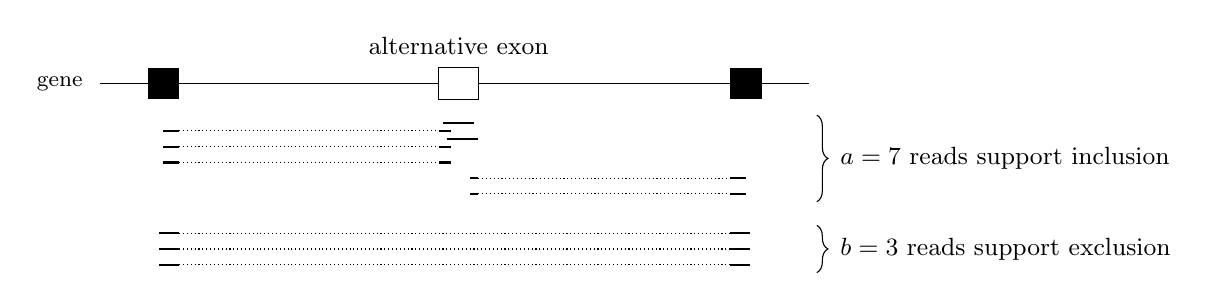
\begin{tikzpicture}[every node/.style={font=\small}]
    \draw (0,0) -- (9,0);
    \fill (0.6,-0.2) rectangle (1.0,0.2);
    \draw[fill=white] (4.3,-0.2) rectangle (4.8,0.2);
    \fill (8.0,-0.2) rectangle (8.4,0.2);
    \node[above] at (4.55,0.25) {alternative exon};
    \node[left, align=right, font=\footnotesize] at (-0.1,0) {gene};
    % inclusion reads
    \foreach \y in {-0.6,-0.8,-1.0} {\draw[thick] (0.8,\y) -- (1.0,\y); \draw[densely dotted] (1.0,\y) -- (4.3,\y); \draw[thick] (4.3,\y) -- (4.45,\y);}
    \foreach \y in {-0.6,-0.8} {\draw[thick] (4.7,\y-0.6) -- (4.8,\y-0.6); \draw[densely dotted] (4.8,\y-0.6) -- (8.0,\y-0.6); \draw[thick] (8.0,\y-0.6) -- (8.2,\y-0.6);}
    \draw[thick] (4.35,-0.5) -- (4.75,-0.5);
    \draw[thick] (4.4,-0.7) -- (4.8,-0.7);
    \draw[decorate, decoration={brace, amplitude=4pt}] (9.1,-0.4) -- (9.1,-1.5) node[midway, right=5pt] {$a=7$ reads support inclusion};
    % exclusion reads
    \foreach \y in {-1.9,-2.1,-2.3} {\draw[thick] (0.75,\y) -- (1.0,\y); \draw[densely dotted] (1.0,\y) -- (8.0,\y); \draw[thick] (8.0,\y) -- (8.25,\y);}
    \draw[decorate, decoration={brace, amplitude=4pt}] (9.1,-1.8) -- (9.1,-2.4) node[midway, right=5pt] {$b=3$ reads support exclusion};
  \end{tikzpicture}
  \caption{Estimating the percent spliced in $\Psi$ of an alternative exon (white) from RNA-seq reads. Reads inside the exon and junction reads to it support inclusion; junction reads joining the flanking constitutive exons (black) support exclusion. After \citet{xiong2015}.}
  \label{fig:psi}
\end{figure}

The counts carry information about uncertainty as well. If each discriminating read independently supports inclusion with probability $\Psi$, then $a\mid\Psi\sim\Bin(a+b,\Psi)$, and with a uniform $\BetaD(1,1)$ prior the posterior is $\Psi\mid a,b\sim\BetaD(a+1,b+1)$, the $K=2$ case of the Dirichlet conjugacy of Section~\ref{sec:dirichlet}. Seven inclusion and three exclusion reads give the same point estimate as 70 and 30, but a much broader posterior (Figure~\ref{fig:psi_beta}). Models trained to predict $\Psi$ should account for this: an exon with few reads gives a noisy target.

\begin{figure}[!htbp]
  \centering
  \includegraphics[width=0.55\linewidth]{psi_beta.pdf}
  \caption{Posterior distribution of $\Psi$ under a binomial model with a uniform prior, for $a=7$ inclusion and $b=3$ exclusion reads, and for ten times as many reads. Both have mode $0.7$; the posterior standard deviations are 0.13 and 0.045.}
  \label{fig:psi_beta}
\end{figure}

\subsection{The splicing code}

\citet{barash2010} and \citet{xiong2015} built models that predict $\Psi$ for an exon in a given tissue from its sequence and that of its neighbourhood, an approach they called the \emph{splicing code}. Training data came from RNA-seq of 16 human tissues, giving $\Psi$ for some ten thousand alternative exons in each. The model of \citet{xiong2015} is close to classical machine learning:
\begin{itemize}
  \item \emph{Targets.} The binomial model gives a distribution over $\Psi$ for each exon and tissue, with additional variance from bootstrap resampling of read positions. The loss is the KL divergence from this target distribution $P(\Psi)$ to the model's predicted distribution $Q(\Psi\mid\vx)$, where $\vx$ are the features, so noisy targets count for less.
  \item \emph{Features.} 1,393 hand-engineered features of the exon, its flanking introns and its neighbouring exons, including the presence of known splicing regulatory elements, splice site strength, \emph{translatability} (whether including or skipping the exon preserves the reading frame or introduces a premature stop codon), evolutionary conservation, and predicted nucleosome positioning.
  \item \emph{Model.} An ensemble of neural networks with two sigmoidal hidden layers, treated as Bayesian neural networks and fit by MCMC.
\end{itemize}
Some features are informative for an unusual reason. The spliceosome cannot check whether an exon preserves the reading frame, or whether its sequence is conserved in chimpanzees. These features are predictive because natural selection has shaped which exons are included: an exon whose inclusion would break the protein is unlikely to be included at high levels in a healthy tissue, and an exon whose sequence is conserved is more likely to be functional. A model using them partly learns the outcome of evolution rather than the mechanism of splicing, which matters when we use it to predict the effect of new mutations. Nucleosome features are relevant for a more mechanistic reason: transcription and splicing are coupled, and nucleosomes are enriched on exons.

The predictions correlate well with measured $\Psi$ across exons (Figure~\ref{fig:xiong}a), although with a sigmoidal bias. Predicting which exons are included is easier than predicting how inclusion of one exon changes between tissues, since differences between tissues are much smaller than differences between exons. A model that maps sequence to splicing can also be used in place of a mutagenesis experiment, as for the models of transcription factor binding in Chapters 2 and 4: run it on the reference and the variant sequence and take the difference $\Delta\Psi$ (Figure~\ref{fig:xiong}b). Applied to hundreds of thousands of genetic variants, predicted effects were largest within exons and in the first few tens of nucleotides of the flanking introns, near the splice sites, although some deeper intronic variants had large predicted effects too. Variants associated with disease had larger predicted effects than common variants, and this held for \emph{synonymous} exonic variants, which do not change the amino acid sequence, as well as for missense variants, which do. A synonymous variant can still change the protein by changing splicing.

\begin{figure}[!htbp]
  \centering
  \begin{subfigure}[b]{0.38\linewidth}
    \includegraphics[width=\linewidth]{slides/xiong_psi_prediction.png}
    \caption{}
  \end{subfigure}\hfill
  \begin{subfigure}[b]{0.6\linewidth}
    \includegraphics[width=\linewidth]{slides/xiong_delta_psi.png}
    \caption{}
  \end{subfigure}
  \caption{The splicing code. (a) Predicted against RNA-seq-measured $\Psi$ for 10,689 test exons in 16 tissues; for each bin of measured $\Psi$ (column) the colour shows the distribution of predictions. (b) Locations and predicted $\Delta\Psi$ of 81,608 disease-annotated intronic and exonic (synonymous or missense) variants, in the 300\,nt of intron and 100\,nt of exon on either side of each splice site; $|\Delta\Psi|$ is truncated at 10\%. Reproduced from \citet{xiong2015}.}
  \label{fig:xiong}
\end{figure}

\subsection{SpliceAI}

SpliceAI~\citep{jaganathan2019} takes a different approach. Rather than predicting the inclusion of known exons from engineered features, it predicts from sequence alone, at every position of a pre-mRNA, whether the position is a splice \emph{acceptor} (the end of an intron), a splice \emph{donor} (the start of an intron) or neither. This is a three-class classification problem at each position, trained with the cross-entropy loss of Chapter 1 against splice sites annotated in GENCODE transcripts, and tested on held-out chromosomes. The input is the one-hot encoded pre-mRNA sequence with up to 5,000\,nt of context on each side of each position. Long context matters because the spliceosome must choose among many candidate sites, and the right choice depends on the surrounding exons, introns and regulatory elements.

\paragraph{Architecture.} SpliceAI is a deep convolutional network built from two ingredients that we met in Chapter 3: residual connections and dilated convolutions (Figure~\ref{fig:resnet_dilated}).

A \emph{residual block}~\citep{he2016} computes $\vx+F(\vx)$ rather than $F(\vx)$, where $\vx$ is the block's input (the network input or the activations of an earlier layer) and $F$ is a small stack of layers. If the weights of $F$ are zero, the block is the identity, so a block can learn to do nothing, and with small initial weights each block starts close to the identity. The identity path also lets gradients pass directly to early layers, the same idea by which LSTM and GRU cells (Chapter 7) improve on a vanilla recurrent network. Residual connections made it possible to train much deeper networks for image recognition~\citep{he2016}. Since $\vx$ and $F(\vx)$ are added, they must have the same dimensions, so operations that change the resolution, such as max pooling, cannot be used inside a block. In SpliceAI each residual block is two repeats of batch normalization~\citep{ioffe2015}, a ReLU and a convolution (Figure~\ref{fig:spliceai_arch}).

A \emph{dilated convolution}~\citep{yu2016} with dilation $d$ applies its filter to input positions $d$ apart. For a one-dimensional input $f$ and a filter $k$ of width $W$, the output at position $t$ is
\begin{equation}
  (k *_d f)_t = \sum_{\tau} k_\tau\, f_{t-d\tau},
\end{equation}
where $\tau$ ranges over the $W$ filter positions; $d=1$ is ordinary convolution. Dilation is different from a stride, which moves the filter by more than one position between outputs and so reduces the resolution. A dilated convolution keeps one output per position but widens the stretch of input each output depends on. A width-$W$ convolution with dilation $d$ extends the receptive field by $(W-1)d$ positions, so increasing the dilation from layer to layer makes the receptive field grow much faster with depth than for ordinary convolutions.

\begin{figure}[!htbp]
  \centering
  \begin{tikzpicture}[>=Stealth, every node/.style={font=\small},
      box/.style={draw, minimum width=2.4cm, minimum height=0.5cm, fill=gray!8}]
    \node at (-1.6,4.4) {(a)};
    \node (x) at (0,4.4) {$\vx$};
    \node[box] (b1) at (0,3.5) {batch norm, ReLU};
    \node[box] (c1) at (0,2.8) {conv $(N,W,D)$};
    \node[box] (b2) at (0,2.1) {batch norm, ReLU};
    \node[box] (c2) at (0,1.4) {conv $(N,W,D)$};
    \node[circle, draw, inner sep=1pt] (plus) at (0,0.5) {$+$};
    \node (out) at (0,-0.3) {$\vx+F(\vx)$};
    \draw[->] (x) -- (b1); \draw[->] (b1) -- (c1); \draw[->] (c1) -- (b2); \draw[->] (b2) -- (c2); \draw[->] (c2) -- (plus); \draw[->] (plus) -- (out);
    \draw[->] (0,4.15) -- (1.8,4.15) -- (1.8,0.5) node[midway, right] {identity} -- (plus);
    \draw[decorate, decoration={brace, mirror, amplitude=4pt}] (-1.35,3.75) -- (-1.35,1.15) node[midway, left=5pt] {$F(\vx)$};
    % (b) dilated stack
    \begin{scope}[xshift=4.2cm, yshift=0.2cm]
      \node at (-0.5,4.2) {(b)};
      \foreach \lay/\lab in {0/input, 1/{$d=1$}, 2/{$d=2$}, 3/{$d=4$}} {
        \foreach \i in {0,...,16} \fill[gray!50] ({\i*0.45},{\lay*1.25}) circle (0.06);
        \node[right, font=\footnotesize] at (7.4,{\lay*1.25}) {\lab};
      }
      % connections for output unit at index 8
      \newcommand{\dconn}[3]{\draw[blue!70!black] ({(#1)*0.45},{(#3)*1.25}) -- ({(#2)*0.45},{(#3)*1.25-1.25});}
      \foreach \j in {-4,0,4} {\dconn{8}{8+\j}{3}}
      \foreach \cc in {4,8,12} {\foreach \j in {-2,0,2} {\dconn{\cc}{\cc+\j}{2}}}
      \foreach \cc in {2,4,6,8,10,12,14} {\foreach \j in {-1,0,1} {\dconn{\cc}{\cc+\j}{1}}}
      \foreach \i in {1,...,15} \fill[blue!70!black] ({\i*0.45},0) circle (0.07);
      \fill[blue!70!black] (8*0.45,3*1.25) circle (0.08);
      \draw[decorate, decoration={brace, mirror, amplitude=4pt}] (0.45,-0.25) -- (15*0.45,-0.25) node[midway, below=4pt, font=\footnotesize] {receptive field $1+2(1+2+4)=15$};
    \end{scope}
  \end{tikzpicture}
  \caption{(a) A residual block as used in SpliceAI: two repeats of batch normalization, ReLU and a convolution with $N$ channels, filter width $W$ and dilation $D$, added to the block input. (b) Three layers of width-3 convolutions with dilations 1, 2 and 4. The output unit (top) depends on 15 input positions; with ordinary convolutions it would depend on 7.}
  \label{fig:resnet_dilated}
\end{figure}

The largest model, SpliceAI-10k, first maps the one-hot input to 32 channels with a width-1 convolution, then applies 16 residual blocks in four groups of four, with filter width and dilation $(W,D)=(11,1)$, $(11,4)$, $(21,10)$ and $(41,25)$ (Figure~\ref{fig:spliceai_arch}). Every block has 32 channels, so the sequence length and channel number never change. In addition, the activations after each group pass through a width-1 convolution and are summed into the output, a skip connection over many blocks. A final width-1 convolution with three output channels and a softmax gives the acceptor, donor and neither probabilities at each position. Each residual block contains two convolutions, so the total receptive field is
\begin{align}
  1 + 2\times 4\times\left[(11-1)\cdot 1 + (11-1)\cdot 4 + (21-1)\cdot 10 + (41-1)\cdot 25\right]
  &= 1 + 8\times 1250 \nonumber\\
  &= 10{,}001
\end{align}
nucleotides, 5,000 on each side of the predicted position. The smaller models SpliceAI-80nt, -400nt and -2k use only the first one, two or three groups, and their receptive fields of 80, 400 and 2,000 nt (plus one) follow from the same calculation.

\begin{figure}[!htbp]
  \centering
  \includegraphics[width=0.48\linewidth]{slides/spliceai_architecture.png}
  \caption{SpliceAI architectures with increasing context. RB$(N,W,D)$ is a residual block with $N$ channels, filter width $W$ and dilation $D$ (inset); Conv$(N,W,D)$ is a convolution. Reproduced from \citet{jaganathan2019}.}
  \label{fig:spliceai_arch}
\end{figure}

\paragraph{Accuracy.} Splice sites are rare, a few per ten thousand positions, so accuracy is measured with metrics suited to class imbalance (Chapter 1). The \emph{top-$k$ accuracy} is computed by setting the threshold so that the number of positions called splice sites equals the actual number of splice sites $k$, and reporting the fraction of those $k$ calls that are correct; it is the precision at the point where precision equals recall. The second metric is the area under the precision-recall curve (PR-AUC). Accuracy increases with context (Table~\ref{tab:spliceai}). The earlier methods in the table use much shorter windows; MaxEntScan~\citep{yeo2004}, for example, scores 9\,nt around a donor and 23\,nt around an acceptor, so the comparison mainly shows how much the wider context helps.

\begin{table}[!htbp]
  \centering
  \caption{Splice site prediction on held-out chromosomes, from \citet{jaganathan2019}.}
  \label{tab:spliceai}
  \begin{tabular}{lcc}
    \toprule
    Model & Top-$k$ accuracy & PR-AUC \\
    \midrule
    SpliceAI-80nt & 0.57 & 0.60 \\
    SpliceAI-400nt & 0.90 & 0.95 \\
    SpliceAI-2k & 0.93 & 0.97 \\
    SpliceAI-10k & \textbf{0.95} & \textbf{0.98} \\
    \midrule
    GeneSplicer & 0.30 & 0.23 \\
    MaxEntScan & 0.22 & 0.15 \\
    NNSplice & 0.22 & 0.15 \\
    \bottomrule
  \end{tabular}
\end{table}

Figure~\ref{fig:spliceai_cftr}a shows predictions across the full pre-mRNA of \textit{CFTR}, the gene mutated in cystic fibrosis, about 189\,kb long with exons that are tiny compared with the introns. At the threshold that calls as many sites as there are true sites, SpliceAI-10k recovers almost all annotated acceptors and donors, while MaxEntScan's calls are scattered through the introns. In silico mutagenesis (Chapter 4) of the sequence around an acceptor (Figure~\ref{fig:spliceai_cftr}b) shows that the model relies on the AG and the polypyrimidine tract and on the GT at the downstream donor, and also on exonic motifs such as GAAGA, which resembles known ESEs.

\begin{figure}[!htbp]
  \centering
  \begin{subfigure}[b]{\linewidth}
    \centering
    \includegraphics[width=0.85\linewidth]{slides/spliceai_cftr.png}
    \caption{}
  \end{subfigure}
  \begin{subfigure}[b]{\linewidth}
    \centering
    \includegraphics[width=0.85\linewidth]{slides/spliceai_saliency.png}
    \caption{}
  \end{subfigure}
  \caption{SpliceAI predictions. (a) The pre-mRNA of \textit{CFTR} scored by MaxEntScan (top) and SpliceAI-10k (bottom); triangles are predicted acceptors (red) and donors (green), and black boxes are the exons. (b) In silico mutagenesis around exon 9 of \textit{U2SURP}: the height of each nucleotide is the decrease in predicted acceptor strength at the black triangle when that nucleotide is mutated. Reproduced from \citet{jaganathan2019}.}
  \label{fig:spliceai_cftr}
\end{figure}

\paragraph{Variant effects.} To score a variant, SpliceAI is run on the reference and the alternative sequence, and the changes in predicted acceptor and donor probabilities at positions near the variant are summarized as four quantities: acceptor gain, acceptor loss, donor gain and donor loss. Their maximum, the $\Delta$ score between 0 and 1, is used to call variants splice-altering. Figure~\ref{fig:spliceai_pygb} shows an example confirmed by RNA-seq. A C$>$T variant in \textit{PYGB} creates a GT that is used as a new donor, shortening the exon by 35\,nt in the individual who carries it. Since 35 is not a multiple of 3, this shifts the reading frame of everything downstream.

\begin{figure}[!htbp]
  \centering
  \includegraphics[width=0.6\linewidth]{slides/spliceai_pygb.png}
  \caption{A variant predicted by SpliceAI to create a donor ($\Delta$ score 0.77) in \textit{PYGB}. RNA-seq coverage and junction read counts (arcs) in an individual carrying the variant (blue) and a control individual (grey); the carrier uses a novel junction 35\,bp upstream of the known donor. Reproduced from \citet{jaganathan2019}.}
  \label{fig:spliceai_pygb}
\end{figure}

\paragraph{De novo mutations in neurodevelopmental disorders.} Autism spectrum disorder (ASD) and intellectual disability (ID) have a substantial contribution from \emph{de novo} mutations, mutations that arose in a parent's germ line and so are present in the child but in neither parent. Each person carries of the order of 70 de novo mutations, most of them harmless; the damaging ones in affected children are enriched in particular genes. \citet{jaganathan2019} scored de novo mutations from exome or genome sequencing of 4,293 individuals with ID from the Deciphering Developmental Disorders study~\citep{mcrae2017} and 3,953 individuals with ASD from the Simons Simplex Collection and the Autism Sequencing Consortium~\citep{turner2016,sanders2015}, and compared them with mutations in unaffected siblings. De novo mutations predicted to disrupt splicing were enriched in cases (Table~\ref{tab:denovo}), and counting them alongside protein-truncating mutations identified additional candidate genes. RNA-seq from affected individuals in the Simons Simplex Collection confirmed aberrant splicing for predicted variants, for example a de novo mutation in \textit{MED13}, a subunit of the Mediator complex that links transcription factors to Pol II.

\begin{table}[!htbp]
  \centering
  \caption{De novo mutations predicted by SpliceAI to disrupt splicing in intellectual disability (ID) and autism spectrum disorder (ASD) cohorts, compared with unaffected controls, as summarized from \citet{jaganathan2019}. The proportion is the estimated share of disease-causing de novo mutations that act through splicing.}
  \label{tab:denovo}
  \begin{tabular}{lcc}
    \toprule
    & ID ($n=4{,}293$) & ASD ($n=3{,}953$) \\
    \midrule
    Fold enrichment & 1.54 & 1.38 \\
    $p$-value & $<0.001$ & $<0.01$ \\
    Proportion of disease mutations & 7\% & 16\% \\
    New candidate genes & 5 & 2 \\
    \bottomrule
  \end{tabular}
\end{table}

Many of the genes implicated in ASD are expressed specifically in neurons and act at synapses, as one might expect, but many others are general regulators of transcription and chromatin, such as \textit{MED13}, expressed in every cell type. One explanation is that neurons, with their complex and long-lived gene expression programs, are especially sensitive to defects in such general machinery.

\subsection{Learning from random sequences}

All the models so far were trained on natural sequences. The human genome is large, but it contains a limited number of exons and introns, and the natural examples are confounded by evolution: as we saw, features such as conservation and translatability are predictive without being mechanisms. \citet{rosenberg2015} instead measured splicing for more than two million synthetic \emph{minigenes}. Each construct has fixed flanking exons and an intron of a few hundred nucleotides, much shorter than a typical human intron because of the cost of synthesizing long DNA, into which one or two random 25\,nt segments are inserted (Figure~\ref{fig:rosenberg}a). In the alternative $5'$ splice site library shown, two donors, SD$_1$ and SD$_2$, compete; the random sequence can strengthen or weaken them, create a new donor inside the random segment (SD$_\text{new}$) or activate a cryptic one (SD$_\text{crypt}$). A random barcode in the downstream exon identifies each construct after the library is transfected into cells and the spliced RNA is sequenced, so the usage of each splice site can be measured for every random sequence.

With this much unconfounded data, simple models work well. The \emph{hexamer additive linear} (HAL) model predicts the log-odds of using one splice site rather than another as a sum of weights, one per $k$-mer per random region, over the $k$-mers present: it is a linear model on $k$-mer counts. Figure~\ref{fig:rosenberg}b shows how accuracy depends on the amount of training data and on $k$. A $k$-mer model has $4^k$ features per region: 64 for $k=3$ and 16,384 for $k=7$. With little data the simplest model, using 3-mers, is most accurate, and it plateaus early because it cannot represent longer motifs. As the training set grows, models with longer $k$-mers overtake it, and with the full data set the 6-mer and 7-mer models are best. This illustrates the bias-variance trade-off of Chapter 1 directly: the best model complexity depends on how much data there is.

\begin{figure}[!htbp]
  \centering
  \begin{subfigure}[b]{\linewidth}
    \centering
    \includegraphics[width=0.6\linewidth]{slides/rosenberg_library.png}
    \caption{}
  \end{subfigure}
  \begin{subfigure}[b]{\linewidth}
    \centering
    \includegraphics[width=0.8\linewidth]{slides/rosenberg_learning_curve.png}
    \caption{}
  \end{subfigure}
  \caption{Learning splicing from random sequences. (a) Design of the alternative $5'$ splice site library: fixed exons (black) and intron, random 25\,nt segments (N$_{25}$) near two competing donors (SD$_1$, SD$_2$), possible new and cryptic donors (red), and a random barcode (N$_{20}$). (b) Learning curves: held-out $R^2$ for predicting SD$_1$ usage with $k$-mer linear models, as a function of the number of training sequences. Reproduced from \citet{rosenberg2015}.}
  \label{fig:rosenberg}
\end{figure}

A model trained on synthetic sequences can be applied to natural ones. On a small set of variants in \textit{BRCA2}, \textit{CFTR} and \textit{SMN2} whose effects on splicing had been measured by RT-PCR, HAL's predicted $\Delta\Psi$ explained much more of the variance than SPANR, the splicing code model of \citet{xiong2015}, with $R^2=0.51$ against $0.17$ (Figure~\ref{fig:hal_spanr}). A linear model with large, unbiased training data beat a neural network trained on natural sequence, which suggests that the quality and diversity of training data, rather than model architecture, was the limiting factor. Neither model is accurate within any one gene, however.

\begin{figure}[!htbp]
  \centering
  \includegraphics[width=0.6\linewidth]{slides/hal_vs_spanr.png}
  \caption{Predicted against measured (RT-PCR) changes in exon inclusion $\Delta\Psi$ for variants in three genes, for HAL, trained on random-sequence libraries, and SPANR~\citep{xiong2015}, trained on natural sequences. Reproduced from \citet{rosenberg2015}.}
  \label{fig:hal_spanr}
\end{figure}

%======================================================================
\section{Long-read RNA sequencing}
\label{sec:longreads}
%======================================================================

The short-read sequencing that made functional genomics a large field, mostly on Illumina instruments, now produces billions of reads per run, but each read is typically about 150\,nt, while human mRNAs are typically a few thousand nucleotides long. That mismatch is why isoform abundances have to be inferred with EM or variational inference. Long-read technologies aim to sequence whole RNA molecules, so that each read is an isoform (Figure~\ref{fig:long_reads}). Pacific Biosciences (PacBio) sequences circularized cDNA molecules repeatedly and combines the passes into an accurate consensus. Oxford Nanopore Technologies (ONT) pulls a DNA or RNA strand through a protein pore embedded in a membrane and infers the sequence from the changes in ionic current as the nucleotides pass through; it can sequence native RNA without reverse transcription. Nanopore reads have higher error rates than Illumina or PacBio reads, but throughput and accuracy have improved quickly, and large long-read RNA-seq data sets have appeared in the last few years. In practice many reads do not span the whole molecule, because of RNA degradation and incomplete reverse transcription; typical read lengths are around 1.5\,kb, enough to cover many but not all isoforms, so quantification still benefits from a model of which isoforms each read is compatible with.

\begin{figure}[!htbp]
  \centering
  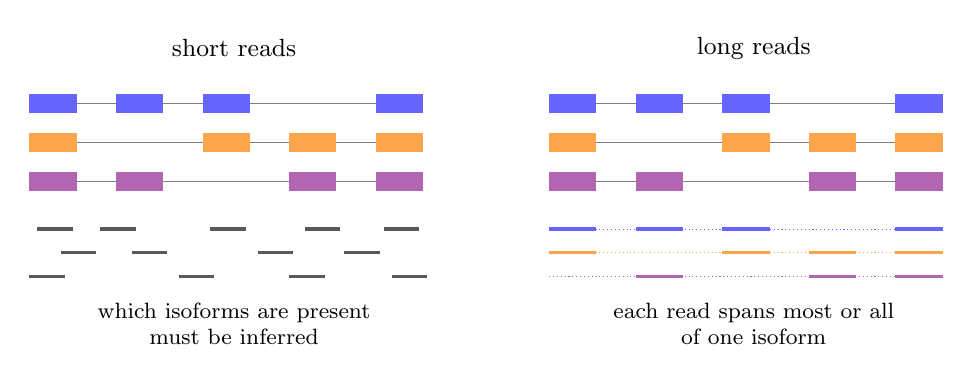
\begin{tikzpicture}[every node/.style={font=\small}]
    \tikzset{ex/.style={minimum width=0.5cm, minimum height=0.25cm, inner sep=0pt}}
    \foreach \side/\xs/\title in {0/0/short reads, 1/6.6/long reads} {
      \begin{scope}[xshift=\xs cm]
        \node at (2.6,1.3) {\title};
        % three isoforms with exons at 0,1,2,3,4 (each 0.6 wide, spacing 1.1)
        \foreach \y/\col/\exs in {0.6/blue!60/{0,1,2,4}, 0.1/orange!70/{0,2,3,4}, -0.4/violet!60/{0,1,3,4}} {
          \draw[gray] (0,\y) -- (5.0,\y);
          \foreach \e in \exs \fill[\col] (\e*1.1,\y-0.12) rectangle (\e*1.1+0.6,\y+0.12);
        }
      \end{scope}
    }
    % short reads
    \foreach \x/\y in {0.1/-1.0, 0.9/-1.0, 2.3/-1.0, 3.5/-1.0, 4.5/-1.0, 0.4/-1.3, 1.3/-1.3, 2.9/-1.3, 4.0/-1.3, 0.0/-1.6, 1.9/-1.6, 3.3/-1.6, 4.6/-1.6}
      \draw[very thick, gray!70!black] (\x,\y) -- (\x+0.45,\y);
    \node[align=center, font=\footnotesize] at (2.6,-2.2) {which isoforms are present\\must be inferred};
    % long reads
    \begin{scope}[xshift=6.6cm]
      \foreach \y/\col/\exs in {-1.0/blue!60/{0,1,2,4}, -1.3/orange!70/{0,2,3,4}, -1.6/violet!60/{1,3,4}} {
        \foreach \e in \exs \draw[very thick, \col] (\e*1.1,\y) -- (\e*1.1+0.6,\y);
        \draw[densely dotted, \col] (0,\y) -- (5.0,\y);
      }
      \node[align=center, font=\footnotesize] at (2.6,-2.2) {each read spans most or all\\of one isoform};
    \end{scope}
  \end{tikzpicture}
  \caption{Short reads (left) cover a small part of an isoform and are often compatible with several; long reads (right) span most or all of a molecule, so its exon structure can be read off directly. The bottom long read is truncated at its $5'$ end, as many real reads are.}
  \label{fig:long_reads}
\end{figure}

Long-read data also enable a new kind of sequence model, one that predicts whole isoforms rather than individual splice sites or exons. \citet{saberi2024} cast this as language modelling. They extend the nucleotide alphabet so that each token records both the nucleotide and its role: uppercase A, C, G, U for exonic positions, lowercase for intronic positions, and four further letters for positions outside the gene. A gene sequence annotated with one isoform's structure then becomes a string, for example \texttt{XWZY\,AUGCAG\,guaagu\ldots{}uucag\,GUUCAA\,ZXWY} for an exon, an intron and a second exon flanked by sequence outside the gene (an invented example), and a model trained to predict the next token, a long-context state-space model of the kind mentioned in Chapter 7, learns jointly which sequences are transcribed and which are spliced out. Trained on long-read data, it can score or sample isoforms for a sequence. One limitation is that the model does not condition on cell type or condition, whereas splicing depends on both. Other approaches, including graph neural networks over the possible exon structures of a gene, are being developed.

%======================================================================
\section{Summary}
%======================================================================

\begin{itemize}
  \item Human genes consist of exons separated by much longer introns. The precursor RNA is capped, spliced and polyadenylated, mostly co-transcriptionally. Splicing removes introns in two steps defined by the GU donor, the branch point A and the AG acceptor.
  \item Alternative splicing, variation in which segments are removed, produces several isoforms per gene. It differs between tissues and development, as for 3R and 4R tau, and is disrupted in many diseases, including cancers driven by splicing factor mutations and neurodegeneration.
  \item Short RNA-seq reads are often compatible with several isoforms. A generative model with a Dirichlet prior on the read proportions $\vtheta$, a discrete latent origin for each read and a read likelihood $p_{nm}=y_{nm}/\tilde L_m$ underlies most quantification methods. EM alternates fractional assignment of reads to isoforms with re-estimation of $\vtheta$ from expected counts.
  \item Variational inference approximates an intractable posterior by the member of a tractable family closest in $\KL(q\|p)$, equivalently maximizing the ELBO. Under a mean-field factorization the CAVI update is $q_i\propto\exp\E_{-i}[\log p]$; for the isoform model it gives a Dirichlet posterior for $\vtheta$ and discrete posteriors for the read origins. CAVI needs conditionally conjugate models, underestimates posterior variance, and needs full passes over the data.
  \item Stochastic variational inference uses Monte Carlo estimates, made differentiable by the reparameterization trick, and minibatches, so that it applies to non-conjugate models and large data.
  \item Splicing can be predicted from sequence. Feature-based models predict exon inclusion $\Psi$; SpliceAI, a deep residual network of dilated convolutions with a 10\,kb receptive field, predicts splice sites at every position and scores the effects of variants, including de novo mutations in neurodevelopmental disorders. Models trained on millions of random sequences show the value of large, unconfounded training data.
  \item Long-read sequencing reads whole isoforms and supports models that predict complete isoform structures from sequence.
\end{itemize}

%======================================================================
\section*{Exercises}
%======================================================================

\begin{enumerate}
  \item Show that the mean of $\Dir(\va)$ is $a_k/a_\cdot$ and its mode is $(a_k-1)/(a_\cdot-K)$ when all $a_k>1$. (Hint: for the mean, use $\Gamma(x+1)=x\Gamma(x)$ and the normalizing constant of a Dirichlet with $a_k$ increased by one.)
  \item Show that the Dirichlet is conjugate to the discrete distribution: if $\vpi\sim\Dir(\va)$ and $t_1,\dots,t_N\mid\vpi\overset{\text{iid}}{\sim}\Disc(\vpi)$, then $\vpi\mid t_{1:N}\sim\Dir(\va+\mathbf{n})$, where $n_k=\sum_n\ind[t_n=k]$.
  \item A gene has two isoforms of effective lengths $\tilde L_1=1000$ and $\tilde L_2=500$. Isoform 2 is isoform 1 with a 500\,nt segment removed. Of $N=150$ reads, 50 fall in the segment unique to isoform 1 and 100 are compatible with both isoforms. Find the maximum likelihood $\vtheta$ by solving the EM fixed point, and convert it to molecule fractions $\tau_m$.
  \item Show that the log likelihood $\sum_n\log\sum_m\theta_m p_{nm}$ is concave in $\vtheta$, and give an example of reads and isoforms for which its maximum over the simplex is not unique.
  \item Derive the ELBO for the CAVI algorithm of Section~\ref{sec:vi} and verify that the terms in $\E[\log\theta_m]$ cancel when $\valpha'=\valpha+\sum_n\vphi_n$.
  \item For a bivariate Gaussian target with correlation $\rho$, show that the mean-field approximation minimizing $\KL(q\|p)$ has variances $\Sigma_{ii}(1-\rho^2)$, and find the mean-field approximation minimizing $\KL(p\|q)$ instead.
  \item Compute the receptive field of SpliceAI-2k from its architecture (Figure~\ref{fig:spliceai_arch}). How many residual blocks of width-11 ordinary (undilated) convolutions would be needed to reach the same receptive field?
  \item Implement EM and CAVI for a simulated three-isoform gene, and compare the CAVI posterior with samples from a Gibbs sampler that alternates $t_n\mid\vtheta$ and $\vtheta\mid t_{1:N}$.
\end{enumerate}
